\documentclass[sigconf,anonymous,review]{acmart}

\usepackage{amsthm}
\usepackage{algorithm}
\usepackage{algorithmic}
\usepackage{multirow}

\AtBeginDocument{%
  \providecommand\BibTeX{{Bib\TeX}}}

% Replace the ACM metadata below with the values supplied by the proceedings venue.
\setcopyright{acmlicensed}
\copyrightyear{2026}
\acmYear{2026}
\acmDOI{XXXXXXX.XXXXXXX}
\acmConference[Conference acronym 'XX]{ACM Conference}{Month DD-DD, 2026}{City, Country}
\acmISBN{978-1-4503-XXXX-X/2026/MM}

\newcommand{\R}{\mathbb{R}}
\newcommand{\method}{\textsc{H2S-NN}}
\newcommand{\ampss}{\textsc{AMPSS}}
\newcommand{\sheafcovpool}{\textsc{SheafCovPool}}
\newcommand{\cF}{\mathcal{F}}
\newcommand{\cL}{\mathcal{L}}
\newcommand{\norm}[1]{\left\lVert #1\right\rVert}
\newcommand{\transpose}{\mathsf{T}}
\newcommand{\concat}{\mathbin\Vert}
\newtheorem{proposition}{Proposition}

\title[H2S-NN]{H2S-NN: Heterogeneous Heterophilic Sheaf Neural Network}

% Replace the affiliation placeholder before submission.
\author{Peeradon Sarnkaew}
\email{peeradonsarnkaew46@gmail.com}
\affiliation{%
  \institution{Independent Researcher}
  \city{Bangkok}
  \country{Thailand}
}
\renewcommand{\shortauthors}{Sarnkaew}

\begin{document}

\begin{abstract}
Learning heterogeneous heterophilic graphs requires addressing two properties. First, heterogeneity represents distinct semantic roles through multiple node and relation types in graphs. Second, heterophily means that connected nodes may differ in labels or features, making similarity-based neighbor aggregation unreliable. Another important aspect is the use of meta-path schemas, which expose typed multi-hop semantics. Many existing meta-path methods represent concrete path instances through endpoint-level views and discard the internal path structure and neglect the higher-order information. Therefore, we introduce the Heterogeneous Heterophilic Sheaf Neural Network (\method{}), which retains the observed graph structure and represents meta-path instances as path-supported \(2D\)-cells, thereby preserving graph heterogeneity. Across the evaluated node-classification, graph-classification, and link-prediction benchmarks, \method{} achieved the strongest overall performance among the compared methods, supporting its effectiveness for heterogeneous heterophilic graph learning.
\end{abstract}

\ccsdesc[500]{Computing methodologies~Neural networks}

\keywords{heterogeneous graph neural networks, heterophily, sheaf neural networks, meta-path instances, diffusion}

\maketitle

\section{Introduction}
\label{sec:introduction}


Heterogeneous graphs are a common representation for modeling complex relational structures, such as citation 
networks \cite{liu2014meta} or social interactions \cite{singh2025overview}. Unlike homogeneous graphs, heterogeneous graphs contain multiple types of nodes and relations with distinct semantic roles \cite{sun2013mining}. Moreover, many graphs are also heterophilic, meaning that adjacent nodes may have different labels or attributes, making simple similarity-based neighbor aggregation unreliable and prone to oversmoothing. A graph can be both heterogeneous and heterophilic, resulting in a much more complex learning task called heterogeneous heterophilic graph learning, as shown in Figure \ref{fig:het_hom_graph}. Furthermore, modeling graphs under the simplifying assumptions of homogeneity or homophily can obscure important structural and relational patterns. These simplifying assumptions can produce an incomplete representation of the original graph and consequently degrade predictive performance \cite{lin2025heterophily}. 

\begin{figure}
  \centering
  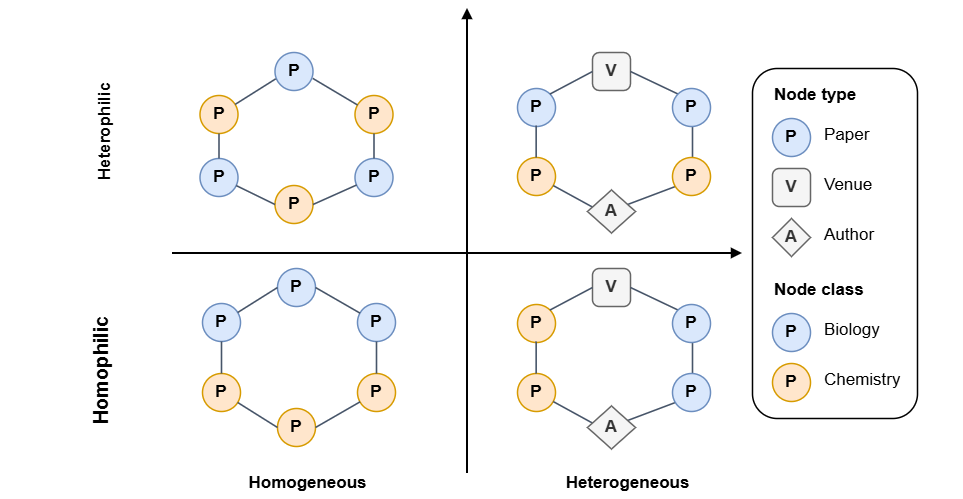
\includegraphics[width=\columnwidth]{figure/Het_HomGraph.drawio.png}
  \caption{An example of a heterogeneous heterophilic graph. The graph contains multiple node and relation types, and adjacent nodes may have different labels or attributes.}
  \label{fig:het_hom_graph}
\end{figure}

Many existing methods address either heterogeneous graphs without explicitly considering heterophily \cite{hu2020heterogeneous,mao2023hinormer,he2024spectral,yang2023simple,wang2019heterogeneous,zhang2019heterogeneous} or heterophilic graphs without modeling heterogeneous node and relation types \cite{grover2025spectro,yue2025graph,bodnar2022neural,ribeiro2026cooperative}. Recent methods have begun to address heterogeneous heterophilic graphs through meta-path-schema-based latent subgraphs \cite{lu2026addressing,chen2025adaptive,li2025hetero2net,guo2023homophily,shen2025heterophily,wang2025homophily}, graph rewiring \cite{tao2025cross}, graph transformers \cite{lin2025heterophily}, and sheaf-based mappings \cite{braithwaite2024heterogeneous}. Another important concept is the use of meta-path schemas. These schemas can express information that is not contained in either node endpoint alone \cite{sun2011pathsim}. For instance, an \texttt{Author-Paper-Author} meta-path schema describes a co-authorship relation in citation networks, as shown in Figure~\ref{fig:meta_path}. However, existing methods either ignore meta-path schemas completely, or use meta-path schemas as semantic views such as filtered edge sets or aggregation channels, rather than retaining each concrete path instance as part of the propagation structure. For example, an \texttt{A-P-A} meta-path schema can connect two authors through a shared paper, but after it is converted into an author-author view, the shared paper and the two authorship edges no longer directly shape the propagation operator. This node-endpoint-only representation is restrictive under heterophily because whether information should be reinforced or contrasted may depend on the relations and intermediate nodes along the path. Collapsing the path can therefore discard local relational structure and higher-order information carried by the concrete path instance.

\begin{figure}
  \centering
  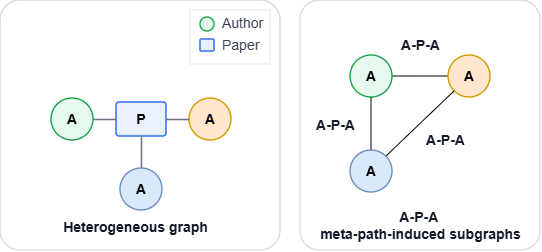
\includegraphics[width=\columnwidth]{figure/meta_path.drawio.png}
  \caption{Illustration of meta-path-schema-induced graph transformation. Under the A-P-A meta-path schema, authors that share a paper in the original heterogeneous graph are connected in an author-level subgraph.}
  \label{fig:meta_path}
\end{figure}

To address this gap, we introduce the \textbf{Heterogeneous heterophilic sheaf neural network (\method{})}, which represents concrete meta-path instances as path-supported \(2D\)-cells and incorporates them into a sheaf-Hodge propagation operator. Compatible node-to-edge and edge-to-face maps preserve the ordered relational context of each path while allowing relation-specific transformations of node and edge states. The \method{} also supports automatic task-aligned selection of meta-paths.
Our main contributions are summarized as follows:
\begin{enumerate}
  \item We propose a Heterogeneous heterophilic sheaf neural network (\method{}), which retains concrete path instances as path-supported \(2D\)-cells in an augmented path-supported 2D cellular complex, thereby preserving both the original graph structure and local relational structure under heterophily.
  \item We develop Adaptive Meta-Path Schema-to-Cell Searching and Selection (\ampss{}), a component of \method{} that selects relevant meta-path schemas and identifies their task-relevant concrete instances.

  \item We develop Sheaf Covariance Pooling (\sheafcovpool{}), a graph-level readout component of \method{} that produces permutation- and gauge-invariant graph representations for graph-level tasks.
\end{enumerate}

As a result, \method{} provides an effective and generalizable model for heterogeneous heterophilic graphs.

\section{Preliminaries}
\label{sec:background}


\subsection{Heterogeneous graphs}

A heterogeneous graph is a tuple $G=(V,E,\phi,\psi)$, where $V$ and $E$ are the node and edge
sets, $\phi:V\rightarrow\mathcal{T}$ assigns each node a type, and
$\psi:E\rightarrow\mathcal{R}$ assigns each edge a relation type. The realized type sets are
$\mathcal{T}=\{\phi(v):v\in V\}$ and $\mathcal{R}=\{\psi(e):e\in E\}$. The graph is heterogeneous
when it contains more than one node type or more than one relation type, i.e.,
$|\mathcal{T}|>1$ or $|\mathcal{R}|>1$; it reduces to a homogeneous graph when
$|\mathcal{T}|=|\mathcal{R}|=1$ \cite{lu2026addressing}.

\subsection{Meta-Path Schemas and Path Instances}
A meta-path schema of length $\ell$ is a typed relation sequence
\begin{equation}
  \pi:
  t_0 \xrightarrow{r_1} t_1 \xrightarrow{r_2}\cdots
  \xrightarrow{r_\ell} t_\ell,
  \qquad t_i\in\mathcal{T},\; r_i\in\mathcal{R},
  \label{eq:background-metapath-schema}
\end{equation}
which specifies a composite relation between its endpoint types \cite{sun2011pathsim}. For each
relation $r$, let $A_r\in\{0,1\}^{|V|\times|V|}$ be its adjacency matrix, with
$(A_r)_{uv}=1$ when a relation of type $r$ connects $u$ to $v$. The schema induces the walk-count
matrix
\begin{equation}
  A_\pi=A_{r_1}A_{r_2}\cdots A_{r_\ell},
  \label{eq:background-metapath-adjacency}
\end{equation}
where $(A_\pi)_{uv}$ counts the concrete walks from $u$ to $v$ that follow $\pi$. When
$t_0=t_\ell$, thresholding $A_\pi$ produces a homogeneous endpoint graph on which
Eq.~\eqref{eq:background-edge-homophily} can be evaluated. For example, as shown in
Figure~\ref{fig:meta_path}, the
paper-author-paper schema has $A_{\mathrm{PAP}}=A_{\mathrm{PA}}A_{\mathrm{AP}}$ and connects
papers that share an author. A concrete path instance is an ordered sequence
$f=(v_0,e_1,v_1,\ldots,e_\ell,v_\ell)$ satisfying $\phi(v_i)=t_i$ and $\psi(e_i)=r_i$. Thus,
$\pi$ describes a type-level pattern, whereas $f$ identifies one occurrence of that pattern in
the observed graph.

\subsection{Homophily and Heterophily}
Homophily refers to the prevalence of edges between nodes that share the same label. For a graph
$G'=(V',E')$ whose endpoint labels are comparable, its edge homophily is
\begin{equation}
  H_{\mathrm{edge}}(G')
  = \frac{1}{|E'|}\sum_{(u,v)\in E'}\mathbf{1}[y_u=y_v],
  \label{eq:background-edge-homophily}
\end{equation}
where $y_u$ is the label of node $u$ and $\mathbf{1}[\cdot]$ is the indicator function
\cite{zhu2020beyond}. Heterophily is the complementary tendency for adjacent nodes to have
different labels. In a heterogeneous graph, labels are generally comparable only after a meta-path
induces an endpoint graph whose nodes share the target type.

We therefore characterize heterogeneous node-classification graphs using metapath-based label
heterophily (MLH) \cite{lin2025heterophily}. Let $\mathcal{P}_2(A)$ be the set of valid
length-two meta-path schemas that start and end at the target node type $A$, and let $G'_p$ denote
the endpoint graph induced by $p\in\mathcal{P}_2(A)$. For each $G'_p$, define edge heterophily as
\begin{equation}
  H_{\mathrm{het}}(G'_p)=1-H_{\mathrm{edge}}(G'_p).
  \label{eq:background-edge-heterophily}
\end{equation}
We use the mean aggregation function over these induced graphs:
\begin{equation}
    \operatorname{MLH}(G;A)
    =
    \frac{1}{|\mathcal{P}_2(A)|}
    \sum_{p \in \mathcal{P}_2(A)}
    H_{\mathrm{het}}(G'_p).
    \label{eq:overall-mlh}
\end{equation}
This mean gives each available semantic view equal weight, rather than allowing a dense induced
graph to determine the dataset-level value. MLH lies in $[0,1]$: values close to $0$ indicate
homophily, whereas values close to $1$ indicate heterophily. For multilabel targets, two endpoint
labels match only when their complete label vectors are equal.

\subsection{Cellular Sheaves and Sheaf Neural Networks}

Based on sheaf theory, a graph can be viewed as a one-dimensional cellular complex, with nodes as \(0\)-cells and edges as
\(1\)-cells. More general cellular complexes may include higher-dimensional cells, such as
\(2D\)-cells bounded by edges, but most sheaf neural networks on graphs operate on the node-edge
complex. We write \(c\unlhd\tau\) when a lower-dimensional cell \(c\) is incident to a
higher-dimensional cell \(\tau\).

A cellular sheaf \(\cF\) assigns each cell \(c\) a vector space, or \emph{stalk},
\(\cF(c)\), and each incident pair \(c\unlhd\tau\) a linear restriction map
\(F_{c\unlhd\tau}:\cF(c)\rightarrow\cF(\tau)\). On a graph \(G=(V,E)\), node and edge
assignments form the cochain spaces
\begin{equation}
  C^0(G,\cF)=\bigoplus_{v\in V}\cF(v),
  \qquad
  C^1(G,\cF)=\bigoplus_{e\in E}\cF(e).
\end{equation}
For an oriented edge \(e=(u\rightarrow v)\), the first coboundary operator
\(\delta_0:C^0(G,\cF)\rightarrow C^1(G,\cF)\) compares endpoint signals after transport into the
edge stalk:
\begin{equation}
  (\delta_0x)_e
  =
  F_{v\unlhd e}x_v-F_{u\unlhd e}x_u.
  \label{eq:prelim-delta0}
\end{equation}
The corresponding sheaf Laplacian is
\(L_0=\delta_0^{\transpose}\delta_0\), with energy
\(x^{\transpose}L_0x=\lVert\delta_0x\rVert_2^2\). When all stalks are one-dimensional and all
restriction maps are identities, \(L_0\) recovers the ordinary graph Laplacian.

Sheaf neural networks can address oversmoothing \cite{cai2020note}, oversquashing \cite{alon2021bottleneck}, and heterophily by replacing direct
feature averaging with diffusion through local stalks and learned restriction maps
\cite{hansen2020sheaf,bodnar2022neural}, leading to numerous recent extensions and applications of sheaf neural networks on graphs and in other domains
\cite{barbero2022sheaf,hernandez2024jointdifsheaf,fiorini2025sheaves,mule2025directional,ribeiro2026cooperative,purificato2025sheaf4rec}. HetSheaf further adapts sheaf maps to heterogeneous graphs \cite{braithwaite2024heterogeneous}.  However, these models
define sheaf structure primarily over observed node-edge incidences. In contrast, \method{} retains selected concrete path instances as path-supported \(2D\)-cells in an augmented path-supported \(2D\)-cellular complex and constructs compatible edge-to-face maps, enabling diffusion over an explicit edge cochain.

\section{Methodology}
\label{sec:method}

\subsection{Problem Formulation}

We consider supervised prediction on a directed heterogeneous graph in which neighboring nodes may have different labels or features. The graph is formulated as
\(G=(V,E,\phi,\psi,X^{\mathrm{raw}})\), where
\(\phi:V\rightarrow\mathcal{T}\) assigns node types,
\(\psi:E\rightarrow\mathcal{R}\) assigns relation types, and
\(X^{\mathrm{raw}}=\{x_v^{\mathrm{raw}}\}_{v\in V}\) contains type-dependent node features with
\(x_v^{\mathrm{raw}}\in\R^{d_{\phi(v)}}\). 

The model is given meta-path schemas
\(\pi\), either supplied manually or selected by \ampss{}.  A schema
\(\pi=(t_0,r_1,t_1,\ldots,r_\ell,t_\ell)\) specifies a valid typed relation sequence, while
\(f=(v_0,e_1,v_1,\ldots,e_\ell,v_\ell)\) denotes one concrete path instance satisfying
\(\phi(v_i)=t_i\) and \(\psi(e_i)=r_i\).  Let \(\mathcal{I}_\pi\) be the set of observed
instances of schema \(\pi\), and let
\(\mathcal{I}_\Sigma=\bigcup_{\pi\in\Sigma}\mathcal{I}_\pi\).  Unlike methods that collapse a
meta-path schema into an endpoint-level homogeneous graph, we represent each retained path instance as a path-supported \(2\)-cell: a face-like higher-order structure whose boundary preserves the ordered path
edges and includes a synthetic closure edge introduced below.

The learning problem is to construct a predictor
\[
  \hat{y}_o
  =
  g_\theta(o;G,\mathcal{I}_\Sigma),
\]
for a task-specific supervised object \(o\).  For node classification, \(o\) is a target node; for
link prediction, \(o\) is a candidate typed node pair; and for graph classification, \(o\) is an
entire graph.  Given labeled training objects \(\mathcal{S}_{\mathrm{train}}\), the parameters are
learned by minimizing
\[
  \min_\theta
  \frac{1}{|\mathcal{S}_{\mathrm{train}}|}
  \sum_{o\in\mathcal{S}_{\mathrm{train}}}
  \mathcal{L}\!\left(g_\theta(o;G,\mathcal{I}_\Sigma),y_o\right).
\]

\(\cL\) is cross-entropy for single-label node and graph classification,
and binary cross-entropy for multilabel node classification and link prediction. Thus, the central challenge is to learn type-aware and relation-aware propagation operators that can use selected concrete path instances as path-supported \(2D\)-cells on heterogeneous heterophilic graphs.

\subsection{Overview}

We introduce \method{}, a Heterogeneous heterophilic sheaf neural network, for supervised learning on heterogeneous heterophilic graphs. As shown in Figure~\ref{fig:pipeline}, \method{} consists of four stages. First, \emph{Input graph preprocessing} prepares typed graph features and relations. Second, \ampss{} generates candidate meta-path schemas using bounded
depth-first search, selects a task-relevant schema set (Stage I), and learns schema-conditioned weights for its retained concrete instances (Stage II). Third, the \emph{Sheaf-Hodge Encoding} stage incorporates the selected concrete path instances to learn node-to-edge and path-supported edge-to-face geometry. Finally, the \emph{Sheaf-Hodge Diffusion} stage evolves the node and edge cochains to obtain their final representations, with the proposed \sheafcovpool{} provided as the graph-level readout. Together, these stages allow \method{} to retain the local relational structure of selected concrete path instances while learning from heterogeneous graphs under heterophily.

\begin{figure*}[htbp]
  \centering
  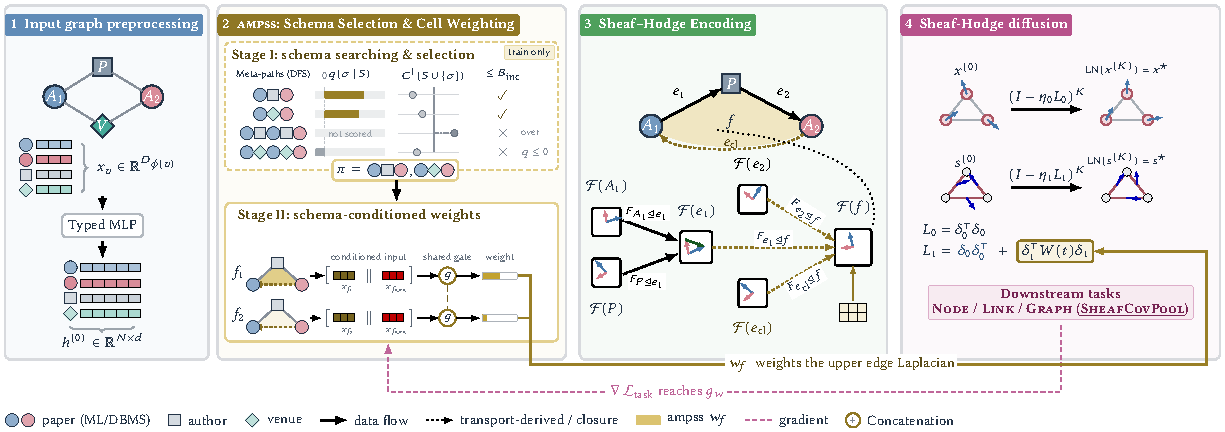
\includegraphics[width=\textwidth]{figure/h2snn_overview.pdf}
  \caption{Overview of \method{} on a citation graph.
\textbf{(1)} Type-specific encoders map heterogeneous node features to a common
\(d\)-dimensional stalk representation.
\textbf{(2)} \ampss{} uses DFS to enumerate meta-path candidates and an auxiliary linear selection model fitted only on the training data to select meta-path schemas in Stage I. In Stage II, it learns schema-conditioned weights for the retained concrete path instances.
\textbf{(3)} Each selected simple path instance is completed by a synthetic
closure \(1\)-cell to form a path-supported \(2D\)-cell. Learned node-to-edge
maps on observed edges define path transports, which construct the closure
restrictions and compatible edge-to-face maps in the corresponding face-stalk
frame.
\textbf{(4)} Node and edge cochains undergo \(K\) parallel Hodge-diffusion steps before task-specific prediction. The learned instance weights modulate the face-induced edge interactions, allowing the supervised task loss to update \ampss{} jointly with the predictor.}
  \Description{A four-panel left-to-right diagram.  Panel one draws a small typed graph and feature
  bars of unequal width becoming bars of equal width d.  Panel two draws a type graph, four
  candidate meta-path schemas with selection-gain bars of which two are kept, and below it two
  concrete path instances of the same schema shaded by their learned weights.  Panel three draws one
  concrete path instance as a shaded polygon closed by a dashed closure edge; below it a node stalk feeds an
  edge stalk, and the stalks of all three boundary edges fan into a single face stalk through
  transports generated by one matrix $A_f$.  Panel four
  draws two parallel diffusion lanes for node and edge cochains and three task heads.  A gold line
  carries the face weight into the upper edge Laplacian and a dashed pink line carries the gradient
  back to the instance-weighting network.}
  \label{fig:pipeline}
\end{figure*}



\subsection{Input Graph Preprocessing: Initialization of Node Stalks and Sheaf Restrictions}

\method{} first maps type-dependent node features into a shared \(d\)-dimensional local feature space (stalk space). This makes representations from different node types compatible with relation-specific restrictions, which transform the endpoint representations into a common edge-stalk space before their disagreement is computed. For each node \(v\), we compute
\begin{equation}
  h_v^{(0)}
  =\operatorname{Dropout}\!\left[
    \operatorname{GELU}\!\left(
      \operatorname{LN}
      \left(W_{\phi(v)}x_v^{\mathrm{raw}}+b_{\phi(v)}\right)
      +q_{\phi(v)}
    \right)
  \right]\in\R^d ,
  \label{eq:node-encoder}
\end{equation}
where \(W_t\) and \(b_t\) are type-specific parameters and \(q_t\) is a learned type embedding. When raw attributes are unavailable, we use a trainable node embedding \(e_v\in\mathbb{R}^{d}\) directly as the initial representation \(h_v^{(0)}\). We initialize the node cochain as \(x^{(0)}=h^{(0)}\) and associate each relation \(r\) with an embedding \(\zeta_r\in\R^{d_r}\).

For an oriented typed edge \(e=(u\xrightarrow{r}v)\), two relation-conditioned networks infer the endpoint restrictions
\(F_{u\unlhd e},F_{v\unlhd e}\in\R^{d\times d}\) from
\(h_u^{(0)}\), \(h_v^{(0)}\), and \(\zeta_r\). The source and target restrictions use the same parameterization:
\begin{equation}
  F_{z\unlhd e}=\lambda_{z,e}Q_{z,e},
  \qquad
  Q_{z,e}^{\transpose}Q_{z,e}=I,
  \qquad
  \lambda_{z,e}>0,
  \quad z\in\{u,v\}.
  \label{eq:conformal-map}
\end{equation}
Here, the orthogonal factor aligns endpoint coordinates, while the positive scale modulates the magnitude of the relation-aware disagreement computed by \(\delta_0\), rather than comparing raw features directly.

We initialize the collection of edge representations (edge cochain) independently from this disagreement:
\begin{equation}
  s_e^{(0)}
  =\operatorname{MLP}_{\mathrm{init}}\!\left(
    h_u^{(0)}\concat h_v^{(0)}\concat \zeta_r
    \concat(\delta_0h^{(0)})_e
  \right).
  \label{eq:edge-init}
\end{equation}
Thus, \(s^{(0)}\) is not restricted to \(\operatorname{im}\delta_0\), allowing the subsequent node-mediated and face-induced edge interactions to act on edge-level information that is not induced solely by node representations. After the selected path instances introduce closure \(1\)-cells, the same coboundary and initialization rules are evaluated over the extended edge set.
\subsection{\ampss{}: Adaptive meta-path schema-to-cell searching and selection}
\label{sec:ampss}

AMPSS is a supporting mechanism for constructing a task-specific set of meta-path instances. \ampss{} has two stages. Stage I generates candidate meta-path schemas
through bounded depth-first search and selects a task-aligned subset of meta-path schemas from the training data. Stage II assigns schema-conditioned weights to the retained path instances, controlling their contribution to the face-induced edge operator. Thus, Stage I selects typed path patterns, whereas Stage II adapts the influence of individual instances to the
supervised task.

\subsubsection{Stage I: task-aligned schema searching and selection.}
Stage I identifies a compact set of task-relevant meta-path schemas. We
construct a type graph from the relation types available during Stage I and
use bounded depth-first search to generate a candidate pool \(\Pi\) of
schemas \(\pi=(t_0,r_1,t_1,\ldots,r_\ell,t_\ell)\), with lengths between
\(\ell_{\min}\) and \(\ell_{\max}\). Candidates with no feasible simple path
instances are discarded. An edge-face incidence is one occurrence of a boundary edge in a path-supported \(2\)-cell.

For a trial schema set \(S\subseteq\Pi\), deterministic instance and
incidence quotas define the retained instances
\(\mathcal{I}_\pi^q(S)\). These instances provide features derived from the retained path instances of each schema
for an auxiliary linear selection model and determine the structural cost.
Stage I greedily selects schemas subject to a schema limit and instance and
incidence budgets.

The structural cost is the number of retained edge-face incidences:
\begin{equation}
  C^{\mathrm{I}}(S)
  =
  \sum_{\pi\in S}
  \sum_{f\in\mathcal{I}_\pi^q(S)}
  (\ell_f+1),
  \label{eq:stage1-cost}
\end{equation}
%where each path instance contributes \(\ell_f\) path-edge incidences and one
%closure-edge incidence. For graph classification, quotas are applied to each
%training graph and the cost is averaged over the training fold.
where each instance contributes its \(\ell_f\) path edges and one closure edge. Thus, the
incidence budget directly bounds the support of the resulting face-induced edge operator.

The auxiliary linear selection model is fitted on an inner-training
partition and evaluated on a disjoint held-out selection partition. The
gain from adding a candidate schema \(\pi\) is
\begin{equation}
\begin{aligned}
q(\pi \mid S)
&=
\cL_{\mathrm{sel}}(S)
-
\cL_{\mathrm{sel}}(S\cup\{\pi\}),
\qquad
\pi \in \mathcal{A}(S),
\\[3pt]
\mathcal{A}(S)
&=
\left\{
\pi \in \Pi \setminus S
\;\middle|\;
\begin{aligned}
|S\cup\{\pi\}| &\le K_\Sigma,\\
C^{\mathrm{I}}(S\cup\{\pi\}) &\le B_{\mathrm{inc}}
\end{aligned}
\right\}.
\end{aligned}
\label{eq:selection-gain}
\end{equation}
Starting from \(S=\varnothing\), Stage I adds the feasible schema that yields
the largest positive reduction in held-out selection loss. The selection
model is refitted for each trial set using labels from the outer training
split only. For link prediction, inner-selection positive links and their
reverse counterparts are excluded from the graph used for selection. After
selection, the retained instances are constructed on the full outer-training
graph. Because schema selection is discrete, gradients from the \method{}
task loss do not update Stage I. Thus, Stage I provides a task-aligned
schema set for Stage II.

\subsubsection{Stage II: schema-conditioned instance weighting.}
For the schema pool selected in Stage I, Stage II assigns a positive weight
to each retained concrete path instance. Instances sharing the same meta-path
schema can encode different task-relevant information. Let \(\xi_f\) denote
the representation of a retained instance \(f\) produced by the ordered path
encoder before constructing its edge-to-face map \(A_f\), and let
\(e_{\pi(f)}\) denote the embedding of the schema of \(f\). We define
\begin{equation}
  w_f(\tau)
  =
  (1-r(\tau))
  +
  2r(\tau)\,
  \operatorname{sigmoid}\!\left(
    g_w(\xi_f\concat e_{\pi(f)})
  \right),
  \label{eq:instance-weight}
\end{equation}
where \(r(\tau)\in[0,1]\) is a warm-up schedule that gradually changes the weights from uniform to learned values. The output layer of \(g_w\) is
initialized at zero; hence, \(w_f(\tau)=1\) at initialization, and learning
starts from the unweighted face-induced edge interactions. The schema embedding enables
the weighting function to distinguish instances from different schemas, such
as \texttt{PAP} and \texttt{PSP}, whereas \(\xi_f\) distinguishes instances
within the same schema. The weights are learned solely through the supervised
task loss.

Let \(W(\tau)=\mathrm{diag}(w_f(\tau))\). Stage II weights the
face-induced component of the edge operator as
\(\delta_1^{\transpose}W(\tau)\delta_1\). Because \(w_f(\tau)>0\), this
component remains positive semidefinite. The weights therefore modulate only
the contribution of retained path-supported \(2D\)-cells. Closure edges remain
part of the extended edge domain and continue to contribute to
\(\delta_0\), \(L_0\), the node-mediated component of the edge operator, the
weighted face boundary in \(\delta_1\), and the edge readout.

Thus, Stage II provides task-driven, instance-level modulation of the selected path-supported \(2D\)-cells while preserving the extended edge structure.

\subsection{Sheaf-Hodge Encoding}

Because nodes, edges, and selected concrete path instances must be incorporated into the sheaf geometry before they can influence diffusion, we introduce a Sheaf-Hodge encoding to address this requirement. It augments the observed graph with path-supported \(2D\)-cells and defines compatible node-to-edge and edge-to-face restriction maps, preserving the ordered structure of each selected path while enabling node and edge cochains to exchange information through observed relations and retained higher-order supports.

\subsubsection{Augmented Path-Supported \(2\)-Cell Construction}

The Sheaf-Hodge encoder augments the observed graph with retained concrete
path instances. In \ampss{} mode, Stage I selects the corresponding
meta-path schemas and determines the retained instances through its
quotas. Rather than replacing an instance with an endpoint-only relation,
\method{} retains the ordered path and augments it with a synthetic closure \(1\)-cell
\[
  f=(v_0,e_1,v_1,\ldots,e_\ell,v_\ell)
\]
as a path-supported \(2D\)-cell whose boundary preserves the ordered path
edges.

Because this path is open, we introduce a synthetic closure \(1\)-cell,
\(e_{\mathrm{cl}}=(v_\ell\rightarrow v_0)\), to form the closed boundary
\begin{equation}
  \partial f=(e_1,\ldots,e_\ell,e_{\mathrm{cl}}).
  \label{eq:face-boundary}
\end{equation}
The closure \(1\)-cell is computationally active in the extended edge domain. Its restriction maps are determined by path transport rather than learned independently.

Let \(E_{\mathrm{cl}}\) contain one closure \(1\)-cell for each retained
instance, and let \(E_{\mathrm{ext}}=E\sqcup E_{\mathrm{cl}}\). The retained
instance set is
\[
\mathcal{I}_{\mathrm{ret}}
=
\bigcup_{\pi\in S}\mathcal{I}_\pi^q(S),
\]
where \(S\) denotes the selected schema set. With \(d\)-dimensional node,
edge, and face stalks, the cochain spaces are
\begin{equation}
  C^0(\cF)=\bigoplus_{v\in V}\cF(v),
  \;
  C^1(\cF)=\bigoplus_{e\in E_{\mathrm{ext}}}\cF(e),
  \;
  C^2(\cF)=\bigoplus_{f\in\mathcal{I}_{\mathrm{ret}}}\cF(f).
  \label{eq:extended-cochains}
\end{equation}

After the closure restrictions are defined by the path transport described
below, the first coboundary in Equation~\eqref{eq:prelim-delta0} is evaluated
over \(E_{\mathrm{ext}}\). Hence, closure \(1\)-cells are included in the extended edge domain and
participate in the initial edge cochain and in both \(L_0\) and \(L_1\). We next define the edge-to-face restriction maps for these path-supported \(2D\)-cells in the following section.

\subsubsection{Path-Supported Edge-to-Face Maps}
\label{sec:face-geometry}

The edge-face construction turns each selected concrete path instance into a path-supported \(2D\)-cellular graph. For a selected \(P\!-\!A\!-\!P\) instance, for example, the two paper-author edges remain the boundary
edges of one path-supported \(2D\)-cell.  The intermediate author remains part of the operator through the ordered path boundary, while the synthetic closure edge adds a path-transport-constrained coupling between the endpoints.  This lets the face-induced edge interactions
couple disagreements along the whole paper-author-paper pattern.

For a general instance \(f=(v_0,e_1,v_1,\ldots,e_\ell,v_\ell)\), \method{} first predicts one free
map \(A_f\in\R^{d\times d}\) from the ordered path.  Each face group contains path instances of a single schema, so all instances
in the group have the same length \(\ell\) and relation sequence
\((r_1,\ldots,r_\ell)\).  The default face encoder concatenates the node states in path order
together with the schema's relation embeddings:
\begin{equation}
A_f
=
\operatorname{MLP}_{\ell}\!\left(
  h_{v_0}^{(0)}\concat\cdots\concat h_{v_\ell}^{(0)}
  \concat \zeta_{r_1}\concat\cdots\concat \zeta_{r_\ell}
\right)
\in\mathbb{R}^{d\times d}.
  \label{eq:face-map}
\end{equation}
Here, \(\operatorname{MLP}_{\ell}\) is a path-length-specific MLP that maps
the ordered path representation to the entries of \(A_f\). The resulting map
\(A_f\) defines the local coordinate system of the face stalk for instance
\(f\).
We construct the edge-to-face maps by transporting \(A_f\) along the ordered
path through the node-to-edge restriction maps. This construction ensures
that the face-induced component measures edge-level inconsistency around a
selected path-supported \(2\)-cell, rather than creating an artificial face
signal from an edge cochain induced solely by node representations. Starting
from the base vertex \(v_0\), the transport is
\begin{equation}
  \begin{aligned}
  T_{v_0}&=A_f,
  \qquad
  T_{v_i}=T_{v_{i-1}}F_{u\unlhd e_i}^{-1}F_{v\unlhd e_i},\\
  F_{e_i\unlhd f}&=T_{v_{i-1}}F_{u\unlhd e_i}^{-1},
  \end{aligned}
  \label{eq:transport}
\end{equation}
where \(u=v_{i-1}\) and \(v=v_i\).  

%Because each restriction map is a positive scale times an orthogonal matrix, its inverse has the closed form \(F^{-1}=F^\transpose/\lambda^2\).

The closure edge uses the same path transport:
\begin{equation}
  F_{v_0\unlhd e_{\mathrm{cl}}}=I,
  \qquad
  F_{v_\ell\unlhd e_{\mathrm{cl}}}=T_{v_0}^{-1}T_{v_\ell},
  \qquad
  F_{e_{\mathrm{cl}}\unlhd f}=A_f .
  \label{eq:closure-maps}
\end{equation}
The middle map is the transformation accumulated along the path \(\prod_i F_{u\unlhd e_i}^{-1}F_{v\unlhd e_i}\).  Hence, the closure edge introduces no additional learned restriction map.

Let \(\eta(e,f)\in\{-1,+1\}\) denote the incidence orientation. The weighted second coboundary is
\begin{equation}
  (\delta_{1,w}s)_f
  =
  \sqrt{w_f}
  \sum_{e\in\partial f}
    \eta(e,f)F_{e\unlhd f}s_e .
  \label{eq:delta1}
\end{equation}
Writing
\(B_fs=\sum_{e\in\partial f}\eta(e,f)F_{e\unlhd f}s_e\),
the corresponding face-induced contribution is
\begin{equation}
  \delta_{1,w}^{\transpose}\delta_{1,w}
  =
  \sum_{f\in\mathcal{I}_{\mathrm{ret}}}
    w_f B_f^{\transpose}B_f .
  \label{eq:weighted-up}
\end{equation}

\begin{proposition}[Exact cochain condition]
\label{prop:chain}
For every path instance constructed by \method{} whose node sequence is a
simple path and whose boundary follows the default forward orientation, the
maps in
Eqs.~\eqref{eq:transport} - \eqref{eq:closure-maps} satisfy
\(\delta_{1,w}\delta_0=0\) identically for every node cochain and every value
of the learned parameters.
\end{proposition}
\begin{proof}
By construction \(F_{e_i\unlhd f}F_{u\unlhd e_i}=T_{v_{i-1}}\) and
\(F_{e_i\unlhd f}F_{v\unlhd e_i}=T_{v_i}\).  The \(i\)-th path term of
\(\delta_{1,w}\delta_0x\) is therefore
\(T_{v_i}x_{v_i}-T_{v_{i-1}}x_{v_{i-1}}\), and summing over the path telescopes to
\(T_{v_\ell}x_{v_\ell}-T_{v_0}x_{v_0}\).  The closure maps give
\(F_{e_{\mathrm{cl}}\unlhd f}F_{v_0\unlhd e_{\mathrm{cl}}}=T_{v_0}\) and
\(F_{e_{\mathrm{cl}}\unlhd f}F_{v_\ell\unlhd e_{\mathrm{cl}}}=T_{v_\ell}\), so the closure term
contributes \(T_{v_0}x_{v_0}-T_{v_\ell}x_{v_\ell}\).  The total sum is zero.  The simple-path
condition is required because the transport assigns one map to each node position; a revisited node,
including a coincident endpoint pair, would require two transported values for the same node.
\end{proof}
The chain condition in Proposition~\ref{prop:chain} is scoped to the implemented simple-path,
transport-composed faces and their aligned closure edges.  Within that scope it is
not optimized as an additional penalty but enforced by construction. Its role is to keep
the interpretation of the Hodge decomposition clean: edge signals in \(\operatorname{im}\delta_0\)
come from edge signals induced by node representations, while the face-induced component acts on edge-level residuals around selected
path-supported cycles.

%\begin{figure}[htbp]
%  \centering
%  \fbox{\rule{0pt}{4.2cm}\rule{0.94\columnwidth}{0pt}}
  %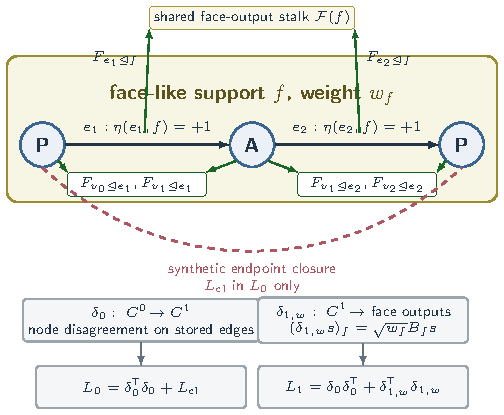
\includegraphics[width=\columnwidth]{figure/h2snn_sheaf_hodge_operator.pdf}
%  \caption{AMPSS-selected path-supported \(2D\)-cells define a sheaf-Hodge operator. Currently in construction.}
%  \label{fig:sheaf-hodge-operator}
%\end{figure}

\subsection{Sheaf-Hodge Diffusion}
\label{sec:closure}

After the restriction maps have been constructed, \method{} diffuses node
and edge cochains using one node operator and one edge operator:
\begin{align}
  L_0x
  &=\delta_0^{\transpose}\delta_0x,
  \label{eq:l0}\\
  L_1s
  &=\underbrace{\delta_0\delta_0^{\transpose}s}_{\text{node-mediated component}}
    +\underbrace{\delta_{1,w}^{\transpose}\delta_{1,w}s}_{\text{face-induced component}} .
  \label{eq:l1}
\end{align}
The node operator \(L_0\) compares transported endpoint signals. The edge diffusion operator \(L_1\) contains a node-mediated component and a face-induced component. The
node-mediated component of \(L_1\) relates edge signals through shared
incident nodes, whereas the face-induced component couples boundary edges
within selected path-supported \(2D\)-cells. In Hodge-theoretic terminology,
these are the lower and upper components of the edge operator, which represent node-mediated and face-induced edge interactions, respectively. Because each closure \(1\)-cell is part of the extended edge
set, it participates in both components without requiring a separate
node-side correction.

Starting from \(x^{(0)}=h^{(0)}\) and the independently initialized edge cochain \(s^{(0)}\),
\(K\) explicit Euler steps give
\begin{equation}
  \begin{aligned}
  x^{(k+1)}&=x^{(k)}-\alpha_0L_0x^{(k)},\\
  s^{(k+1)}&=s^{(k)}-\alpha_1L_1s^{(k)},
  \qquad k=0,\ldots,K-1 .
  \end{aligned}
  \label{eq:diffusion}
\end{equation}
The positive step sizes may be learned.  Node and edge cochains are updated by separate \(L_0\) and \(L_1\) operators. Although updated node and edge states are not exchanged between diffusion steps, both operators share the learned restriction geometry and initial node representations. Layer normalization then gives the terminal states \(x^\star\) and \(s^\star\), which are passed to
the task-specific readout.

The Hodge operators are evaluated through local restriction maps and indexed aggregation without explicitly forming global operators. The implementation batches local restriction maps and aggregates
contributions with indexed sums.  This applies \(\delta_0\), \(\delta_0^{\transpose}\),
\(\delta_{1,w}\), and \(\delta_{1,w}^{\transpose}\) directly to node, edge, and face tensors.

Three implementation boundaries are important.  First, \(\delta_{1,w}\) uses the complete boundary
cycle, consisting of the \(\ell\) path edges and the closure \(1\)-cell.  Second, incidence signs are
represented explicitly.  The paths produced by the current enumeration use \(+1\) signs because the enumeration follows stored edge directions and orients the closure edge along the cycle.  Third, the exact
transport argument assumes simple paths, so instances that revisit a node, including coincident
endpoints, are excluded during enumeration.  Under these constraints, the chain condition is a
property of the constructed operator, not a penalty added to the training objective.

The shared backbone produces final node states \(x^\star\) and edge states \(s^\star\). For node classification, the target-node state is combined with pooled incident-edge information. For link prediction, endpoint representations are formed from node and incident-edge states before applying a pair decoder. For graph classification, \sheafcovpool{} aggregates node and edge
representations into a graph-level vector, as described next.

\subsection{\sheafcovpool{}}

Graph classification requires one representation for the whole graph, yet node and edge states
are expressed in different local coordinate systems. Averaging incident edge coordinates directly
would therefore mix vectors from different spaces. Before pooling, \sheafcovpool{} projects each incident edge state into the corresponding node coordinate space using the transpose of its restriction map:
\begin{equation}
  \widetilde{s}_v^\star
  =
  \frac{1}{\deg_{\mathrm{ext}}(v)}
  \left(
  \sum_{e:\operatorname{src}(e)=v}
  F_{\mathrm{src},e}^{\transpose}s_e^\star
  +
  \sum_{e:\operatorname{tgt}(e)=v}
  F_{\mathrm{tgt},e}^{\transpose}s_e^\star
  \right).
  \label{eq:pool-transport}
\end{equation}
Here \(F_{\mathrm{src},e}\) and \(F_{\mathrm{tgt},e}\) denote the restriction maps from the source
and target nodes of \(e\), respectively, into the edge stalk. \(\deg_{\mathrm{ext}}(v)\) is the
number of incidences at \(v\) over observed and closure edges; an isolated node receives the zero vector.
Both endpoints contribute positively because this quantity summarizes incident context rather than
the orientation-sensitive divergence \(\delta_0^{\transpose}s^\star\). The sums range over the
observed and closure edges, so both types of \(1\)-cell contribute.

The readout then forms three complementary views at each node and edge:
\begin{equation}
  \begin{aligned}
  Z_v^{(0)}
  &=\begin{bmatrix}x_v^\star&h_v^{(0)}&\widetilde{s}_v^\star\end{bmatrix}
    \in\R^{d\times3},\\
  Z_e^{(1)}
  &=\begin{bmatrix}
    (\delta_0x^\star)_e&(\delta_0h^{(0)})_e&s_e^\star
  \end{bmatrix}
    \in\R^{d\times3},\\
   G_i^{(q)}
   &=(Z_i^{(q)})^{\transpose}Z_i^{(q)}
     \in\R^{3\times3},\qquad q\in\{0,1\}.
  \end{aligned}
  \label{eq:pool-views}
\end{equation}
This matrix records the energies and pairwise alignments of the three views while removing their
common orthogonal orientation; we call it a Gram matrix. For an ordered view stack, equality of Gram matrices
characterizes equality up to an orthogonal change of basis.

To see why the transported node view has this property, let \(Q_v,R_e\in O(d)\) be independent
changes of basis in the node and edge stalks. Under the consistent transformation
\begin{equation}
  \begin{aligned}
  F_{v\unlhd e}'&=R_eF_{v\unlhd e}Q_v^{\transpose},
  \qquad s_e^{\star\prime}=R_es_e^\star,\\
  (F_{v\unlhd e}')^{\transpose}s_e^{\star\prime}
  &=Q_vF_{v\unlhd e}^{\transpose}s_e^\star .
  \end{aligned}
  \label{eq:pool-gauge}
\end{equation}
Hence \(Z_v^{(0)}\) transforms by \(Q_v\), while \(Z_e^{(1)}\) transforms by \(R_e\), and both Gram
descriptors remain unchanged. This argument requires orthogonal basis changes; the learned
restrictions themselves may be scaled orthogonal maps.

Nodes and edges serve different roles, so separate networks project their Gram matrices.
Within graph \(g\), attention over these invariant descriptors yields first- and second-order
summaries:
\begin{equation}
  \begin{aligned}
   u_i^{(q)}&=\rho_q(\operatorname{vec}G_i^{(q)})\in\R^{F},\\
   a_i^{(q)}
   &=\frac{\exp(g_q(u_i^{(q)}))}
           {\sum_{j\in\mathcal{C}_q(g)}\exp(g_q(u_j^{(q)}))},\\
   \mu_q(g)&=\sum_{i\in\mathcal{C}_q(g)}a_i^{(q)}u_i^{(q)},\\
   \Sigma_q(g)&=\sum_{i\in\mathcal{C}_q(g)}a_i^{(q)}
     (u_i^{(q)}-\mu_q(g))(u_i^{(q)}-\mu_q(g))^{\transpose}.
  \end{aligned}
  \label{eq:pool-moments}
\end{equation}
Here \(q\in\{0,1\}\), \(\mathcal{C}_0(g)\) is the node set, and \(\mathcal{C}_1(g)\) contains the observed and closure
edges. The mean describes the evidence emphasized by attention, whereas the covariance
records how that evidence varies across the graph. The final graph representation is
\begin{equation}
  \gamma_g=
  \bigl[
  \mu_0(g)\concat\operatorname{triu}(\Sigma_0(g))
  \concat\mu_1(g)\concat\operatorname{triu}(\Sigma_1(g))
  \bigr].
  \label{eq:pool-summary}
\end{equation}
The order of the raw Gram matrix is fixed at three because it is determined by the three
semantic views in each stack, rather than by a freely chosen hidden width. Changing that order
would require adding or removing stalk-valued views and would therefore define a different readout.
We instead control readout capacity through the post-Gram projection width \(F\). The two means and
two upper-triangular covariance vectors give \(\gamma_g\in\R^{F^2+3F}\).
Because every learned score acts on an invariant Gram matrix and every aggregation is
symmetric, \(\gamma_g\) is invariant to node and edge ordering. Given consistently transformed
states and restriction maps, it is also invariant to independent orthogonal changes of basis in
the node and edge stalks.

\begin{figure}[htbp]
  \centering
  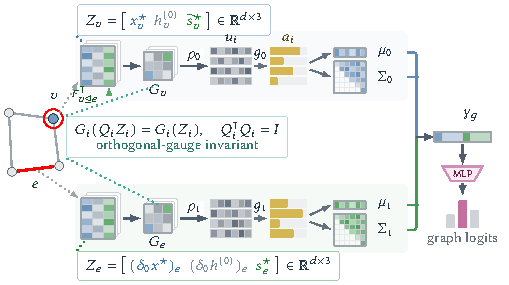
\includegraphics[width=\columnwidth]{figure/sheafcovpool_architecture.pdf}
  \caption{\sheafcovpool{} graph readout. Incident edge states are first expressed in their endpoint node stalks. Node and edge view stacks then become gauge-invariant Gram matrices \(G_i\); attention-weighted means and covariances form the graph representation \(\gamma_g\).}
  \Description{Two parallel lanes, node above and edge below, both fed by the same small graph on
  the left in which every node and edge carries its own local basis.  In each lane a stack of
  three stalk-valued views becomes a three-by-three Gram matrix, a learned projection turns it into
  a token, a learned score turns tokens into attention weights that sum to one within the graph,
  and those weights produce a weighted mean vector and a weighted covariance matrix whose upper
  triangle is kept.  The four summaries concatenate into one vector that an MLP maps to graph
  logits.}
  \label{fig:sheafcovpool}
\end{figure}



\section{Experiments}
\label{sec:experiments}

\subsection{Experiment Settings}
\label{sec:experiment-settings}
To assess the generalizability of \method{} across heterogeneous graph learning settings, we evaluated it on three tasks: node classification, link prediction, and graph classification.
\paragraph{Datasets.}
For node classification, we used three heterogeneous graph benchmarks: DBLP and IMDB from HGB \cite{lv2021hgb} and ACM \cite{wang2019han}. We also calcuated each metapath-based label heterophily (MLH) for each dataset. For graph classification, we selected four datasets from TUDataset \cite{morris2020tudataset}: two biological datasets, PROTEINS and ENZYMES, and two chemical-compound datasets, MUTAG and NCI1. To make the graph heterogeneous, we interpreted the node and edge labels provided by TUDataset as node and relation types, respectively. For link prediction, we used four HGB benchmarks \cite{lv2021hgb}: three user-item interaction networks, LastFM, YouTube, and Amazon, and one biological knowledge graph, PubMed. Dataset statistics are reported in Tables~\ref{tab:node-cls}, \ref{tab:graph-cls}, and~\ref{tab:link-pred}.

\paragraph{Baselines.}
For node classification, we compared \method{} with baselines from four model categories. The homogeneous homophilic baselines comprised GCN \cite{kipf2017gcn}, GAT \cite{velickovic2018gat}, and ChebNetII \cite{he2022chebnetii}, while the homogeneous heterophilic baselines included NSD \cite{bodnar2022neural} and CSNN \cite{ribeiro2026cooperative}. For heterogeneous graphs, we considered the homophilic models HAN \cite{wang2019han}, SeHGNN \cite{yang2023sehgnn}, HiNormer \cite{mao2023hinormer}, and PSHGCN \cite{he2024spectral}, as well as the heterophilic models H2G-former \cite{lin2025heterophily}, Hetero$^2$Net \cite{li2025hetero2net}, H2SGNN \cite{lu2026addressing}, HetSheaf \cite{braithwaite2024heterogeneous}, and LatGRL \cite{shen2025heterophily}.
For graph classification and link prediction, we used a subset of these baselines while retaining representatives from all four categories. Specifically, we included GCN \cite{kipf2017gcn} and GAT \cite{velickovic2018gat} as homogeneous homophilic models; NSD \cite{bodnar2022neural} and CSNN \cite{ribeiro2026cooperative} as homogeneous heterophilic models; HAN \cite{wang2019han} and PSHGCN \cite{he2024spectral} as heterogeneous homophilic models; and H2G-former \cite{lin2025heterophily}, Hetero$^2$Net \cite{li2025hetero2net}, H2SGNN \cite{lu2026addressing}, HetSheaf \cite{braithwaite2024heterogeneous}, and LatGRL \cite{shen2025heterophily} as heterogeneous heterophilic models.
\paragraph{Evaluation Settings.}
For node classification, we followed the HGB benchmark protocol \cite{lv2021hgb}, using transductive training/validation/test splits of 24\%/6\%/70\% and reporting Macro-F1 and Micro-F1. For graph classification, unlike prior work \cite{zhang2018end,amouzad2024graphunet}, we performed 10-fold cross-validation over five random seeds and reported the mean and standard deviation of Macro-F1 and Micro-F1 to evaluate model performance unbiasedly without overestimating model performance. For the multi-class ENZYMES dataset, we adopted a one-vs-rest strategy. For link prediction, we followed the HGB protocol \cite{lv2021hgb}, using transductive splits of 81\%/9\%/10\% and reporting AUPR and AUROC. Negative edges were sampled from the 2-hop neighborhood at a 1:1 ratio to positive edges. All models were trained with early stopping using a patience of 100 epochs. Hyperparameters were selected through per-dataset sweeps, with the complete configurations provided in Appendix~\ref{app:hyperparameters}. We group the baselines according to graph type and homophily assumption as Hom./hom., Hom./het., Het./hom., and Het./het., where the first term indicates whether the graph is modeled as homogeneous or heterogeneous and the second indicates whether the method is designed for homophilic or heterophilic settings. Results are averaged over five random seeds and reported with standard deviations. The code is available at \url{placeholder_for_code_repository.com}.
\subsection{Results}
\label{sec:results}

For the node-classification tasks, the results in Table~\ref{tab:node-cls} show that \method{} achieved the best performance on all three benchmark datasets, outperforming every compared baseline. This demonstrates the effectiveness of \method{} in capturing complex heterogeneous graph structures and relationships, leading to improved node classification performance.

\begin{table*}[htbp]
  \centering
  \caption{Performance on node classification benchmarks measured by Macro-F1 and Micro-F1. Best values are bold. The numbers in parentheses of datasets indicate the homophily ratio.}
  \label{tab:node-cls}
  \scriptsize
  \resizebox{0.8\textwidth}{!}{%
  \begin{tabular}{llcccccc}
    \toprule
    & &
    \multicolumn{2}{c}{DBLP (0.1277)} &
    \multicolumn{2}{c}{ACM (0.2639)} &
    \multicolumn{2}{c}{IMDB (0.7634)} \\
    \cmidrule(lr){3-4}
    \cmidrule(lr){5-6}
    \cmidrule(lr){7-8}
    \textbf{Group} & \textbf{Model}
    & Macro-F1 & Micro-F1
    & Macro-F1 & Micro-F1
    & Macro-F1 & Micro-F1 \\
    \midrule

    \multirow{3}{*}{Hom./hom.}
    & GCN
    & $90.84 \pm 0.32$
    & $91.47 \pm 0.34$
    & $92.17 \pm 0.24$
    & $92.12 \pm 0.23$
    & $57.88 \pm 1.18$
    & $64.82 \pm 0.64$ \\

    & GAT
    & $93.83 \pm 0.27$
    & $93.39 \pm 0.30$
    & $92.26 \pm 0.94$
    & $92.19 \pm 0.93$
    & $58.94 \pm 1.35$
    & $64.86 \pm 0.43$ \\
    
    & ChebNetII
    & $92.05 \pm 0.53$
    & $92.97 \pm 0.48$
    & $92.45 \pm 0.37$
    & $92.33 \pm 0.38$
    & $62.54 \pm 1.29$
    & $68.33 \pm 0.92$ \\

    \midrule

    \multirow{2}{*}{Hom./het.}
    & NSD
    & $92.96 \pm 0.21$
    & $93.42 \pm 0.37$
    & $92.33 \pm 0.78$
    & $92.05 \pm 0.69$
    & $61.61 \pm 0.26$
    & $65.23 \pm 0.51$ \\


    & CSNN
    & $93.73 \pm 0.95$
    & $92.12 \pm 0.19$
    & $93.13 \pm 0.94$
    & $92.81 \pm 0.83$
    & $62.92 \pm 0.34$
    & $62.59 \pm 0.22$ \\


    \midrule

    \multirow{4}{*}{Het./hom.}
    & HAN
    & $91.67 \pm 0.49$
    & $92.05 \pm 0.62$
    & $90.89 \pm 0.43$
    & $90.79 \pm 0.43$
    & $57.74 \pm 0.96$
    & $64.63 \pm 0.58$ \\

    & SeHGNN
    & $95.06 \pm 0.17$
    & $95.42 \pm 0.17$
    & $94.05 \pm 0.35$
    & $93.98 \pm 0.36$
    & $67.11 \pm 0.25$
    & $69.17 \pm 0.43$ \\

    & HiNormer
    & $94.94 \pm 0.21$
    & $94.57 \pm 0.23$
    & $91.87 \pm 0.26$
    & $89.64 \pm 0.39$
    & $67.83 \pm 0.34$
    & $64.65 \pm 0.53$ \\

    & PSHGCN
    & $95.27 \pm 0.13$
    & $95.61 \pm 0.12$
    & $94.35 \pm 0.23$
    & $94.27 \pm 0.23$
    & $72.33 \pm 0.57$
    & $74.46 \pm 0.32$ \\
    \midrule

    \multirow{5}{*}{Het./het.}
    & H2G-former
    & $95.35 \pm 0.81$
    & $95.00 \pm 0.77$
    & $93.99 \pm 0.35$
    & $94.13 \pm 0.87$
    & $59.41 \pm 0.22$
    & $59.63 \pm 0.35$ \\

    & Hetero$^2$Net
    & $94.03 \pm 0.35$
    & $94.46 \pm 0.37$
    & $94.01 \pm 0.54$
    & $93.91 \pm 0.61$
    & $72.33 \pm 0.57$
    & $74.46 \pm 0.32$ \\

    & H2SGNN
    & $95.19 \pm 0.11$
    & $95.56 \pm 0.11$
    & $94.47 \pm 0.25$
    & $94.38 \pm 0.26$
    & $73.04 \pm 0.65$
    & $75.46 \pm 0.43$ \\

    & HetSheaf
    & $93.87 \pm 0.00$
    & $93.77 \pm 0.00$
    & $95.09 \pm 0.00$
    & $94.94 \pm 0.00$
    & $64.65 \pm 0.00$
    & $67.18 \pm 0.00$ \\

    & LatGRL
    & $94.32 \pm 0.44$
    & $94.51 \pm 0.42$
    & $93.47 \pm 0.71$
    & $92.29 \pm 0.43$
    & $58.27 \pm 0.46$
    & $58.81 \pm 0.65$ \\
    \midrule

    Ours
    & \textbf{\method{}}
    & $\mathbf{96.01 \pm 0.58}$
    & $\mathbf{96.31 \pm 0.40}$
    & $\mathbf{95.91 \pm 1.15}$
    & $\mathbf{95.72 \pm 0.68}$
    & $\mathbf{75.05 \pm 0.22}$
    & $\mathbf{76.68 \pm 0.19}$ \\
    \bottomrule
  \end{tabular}%
  }
\end{table*}

Moreover, for the graph classification tasks, table~\ref{tab:graph-cls} shows that \method{} tied the best reported MUTAG score and achieved the highest mean Macro-F1 and Micro-F1 on PROTEINS, ENZYMES, and NCI1 among the compared baselines. This suggests that treating the typed node and edge labels as heterogeneous structure, rather than as plain homogeneous graphs with categorical attributes, remains useful even outside the citation- and social-network domains where heterogeneity is usually studied.

\begin{table*}[htbp]
  \centering
  \caption{Performance on graph classification benchmarks measured by Macro-F1 and Micro-F1. Best values are bold.}
  \label{tab:graph-cls}
  \scriptsize
  \resizebox{0.8\textwidth}{!}{%
  \begin{tabular}{llcccccccc}
    \toprule
    & &
    \multicolumn{2}{c}{MUTAG} &
    \multicolumn{2}{c}{PROTEINS} &
    \multicolumn{2}{c}{ENZYMES} &
    \multicolumn{2}{c}{NCI1} \\
    \cmidrule(lr){3-4}
    \cmidrule(lr){5-6}
    \cmidrule(lr){7-8}
    \cmidrule(lr){9-10}
    \textbf{Group} & \textbf{Model}
    & Macro-F1 & Micro-F1
    & Macro-F1 & Micro-F1
    & Macro-F1 & Micro-F1
    & Macro-F1 & Micro-F1 \\
    \midrule

    \multirow{2}{*}{Hom./hom.}
    & GCN
    & $89.58 \pm 0.63$
    & $90.00 \pm 0.38$
    & $75.92 \pm 0.55$
    & $79.83 \pm 0.49$
    & $12.75 \pm 0.01$
    & $28.33 \pm 0.03$
    & $64.17 \pm 0.29$
    & $64.96 \pm 0.38$ \\

    & GAT
    & $89.58 \pm 0.06$
    & $90.00 \pm 0.96$
    & $75.27 \pm 0.59$
    & $78.38 \pm 0.71$
    & $14.03 \pm 0.05$
    & $16.55 \pm 0.12$
    & $64.17 \pm 0.27$
    & $64.96 \pm 0.69$ \\
    \midrule

    \multirow{2}{*}{Hom./het.}
    & NSD
    & $\mathbf{99.47 \pm 0.53}$
    & $\mathbf{99.69 \pm 0.31}$
    & $73.60 \pm 0.22$
    & $75.89 \pm 0.49$
    & $33.65 \pm 0.37$
    & $35.00 \pm 0.21$
    & $72.30 \pm 0.31$
    & $72.30 \pm 0.10$ \\

    & CSNN
    & $\mathbf{99.21 \pm 0.79}$
    & $\mathbf{99.40 \pm 0.60}$
    & $76.64 \pm 0.28$
    & $77.92 \pm 0.07$
    & $35.15 \pm 0.07$
    & $37.22 \pm 0.13$
    & $74.11 \pm 0.75$
    & $74.30 \pm 0.80$ \\
    \midrule

    \multirow{2}{*}{Het./hom.}
    & HAN
    & $82.91 \pm 0.61$
    & $85.00 \pm 0.19$
    & $79.19 \pm 0.82$
    & $82.22 \pm 0.50$
    & $46.24 \pm 0.06$
    & $45.02 \pm 0.06$
    & $77.60 \pm 0.43$
    & $77.50 \pm 0.29$ \\

    & PSHGCN
    & $94.88 \pm 0.10$
    & $95.00 \pm 0.42$
    & $70.61 \pm 0.13$
    & $72.32 \pm 0.74$
    & $60.18 \pm 0.24$
    & $58.33 \pm 0.38$
    & $74.17 \pm 0.34$
    & $74.96 \pm 0.37$ \\
    \midrule

    \multirow{4}{*}{Het./het.}
    & H2G-former
    & $84.65 \pm 0.71$
    & $85.00 \pm 0.64$
    & $77.64 \pm 0.83$
    & $81.25 \pm 0.65$
    & $58.27 \pm 0.21$
    & $58.33 \pm 0.64$
    & $79.29 \pm 0.61$
    & $79.32 \pm 0.18$ \\

    & Hetero$^2$Net
    & $89.58 \pm 0.16$
    & $90.00 \pm 0.62$
    & $74.66 \pm 0.69$
    & $78.57 \pm 0.43$
    & $61.53 \pm 0.21$
    & $61.36 \pm 0.49$
    & $63.67 \pm 0.66$
    & $65.45 \pm 0.38$ \\

    & H2SGNN
    & $94.88 \pm 0.09$
    & $95.00 \pm 0.35$
    & $70.61 \pm 0.37$
    & $72.32 \pm 0.14$
    & $62.18 \pm 0.44$
    & $61.31 \pm 0.45$
    & $64.17 \pm 0.06$
    & $64.96 \pm 0.44$ \\

    & HetSheaf
    & $\mathbf{100.00 \pm 0.00}$
    & $\mathbf{100.00 \pm 0.00}$
    & $80.56 \pm 0.00$
    & $82.14 \pm 0.00$
    & $62.35 \pm 0.00$
    & $63.33 \pm 0.00$
    & $79.46 \pm 0.00$
    & $79.46 \pm 0.00$ \\

    \midrule

    Ours
    & \textbf{\method{}}
    & $\mathbf{99.65 \pm 0.35}$
    & $\mathbf{99.72 \pm 0.28}$
    & $\mathbf{84.44 \pm 0.21}$
    & $\mathbf{86.23 \pm 0.15}$
    & $\mathbf{64.52 \pm 0.56}$
    & $\mathbf{65.10 \pm 0.37}$
    & $\mathbf{81.22 \pm 0.06}$
    & $\mathbf{81.52 \pm 0.20}$ \\
    \bottomrule
  \end{tabular}%
  }
\end{table*}

The link-prediction results in Table~\ref{tab:link-pred} show that \method{} achieves the best performance on all four link-prediction datasets and all eight reported metrics. This advantage is consistent across multi-node-type graphs (LastFM and
PubMed) and single-node-type, multi-relation graphs (Amazon and YouTube). These results indicate that \method{} supports link prediction on both multi-node-type graphs and single-node-type, multi-relation graphs.

\begin{table*}[htbp]
  \centering
  \caption{Performance on link prediction benchmarks measured by AUPR and AUROC. Best values are bold.}
  \label{tab:link-pred}
  \scriptsize
  \setlength{\tabcolsep}{2.5pt}
  \resizebox{0.8\textwidth}{!}
  {%
  \begin{tabular}{llcccccccc}
    \toprule
    & & \multicolumn{2}{c}{LastFM} & \multicolumn{2}{c}{PubMed} & \multicolumn{2}{c}{Amazon} & \multicolumn{2}{c}{YouTube} \\
    \cmidrule(lr){3-4}\cmidrule(lr){5-6}\cmidrule(lr){7-8}\cmidrule(lr){9-10}
    \textbf{Group} & \textbf{Model} & AUPR & AUROC & AUPR & AUROC & AUPR & AUROC & AUPR & AUROC \\
    \midrule

    \multirow{2}{*}{Hom./hom.}
    & GCN
    & $97.06 \pm 0.48$ & $96.96 \pm 0.41$
    & $96.05 \pm 0.52$ & $92.93 \pm 0.36$
    & $92.40 \pm 0.61$ & $89.66 \pm 0.73$
    & $89.30 \pm 0.39$ & $83.26 \pm 0.52$ \\
    & GAT
    & $63.06 \pm 0.27$ & $51.14 \pm 0.19$
    & $96.07 \pm 0.43$ & $93.27 \pm 0.68$
    & $88.62 \pm 0.34$ & $86.10 \pm 0.45$
    & $66.76 \pm 0.31$ & $58.40 \pm 0.22$ \\
    \midrule

    \multirow{2}{*}{Hom./het.}
    & NSD
    & $97.16 \pm 0.71$ & $96.58 \pm 0.65$
    & $96.41 \pm 0.58$ & $93.65 \pm 0.74$
    & $92.63 \pm 0.49$ & $90.04 \pm 0.38$
    & $89.32 \pm 0.43$ & $83.36 \pm 0.57$ \\
    & CSNN
    & $97.99 \pm 0.42$ & $97.75 \pm 0.39$
    & $96.14 \pm 0.30$ & $92.87 \pm 0.29$
    & $92.10 \pm 0.53$ & $89.62 \pm 0.41$
    & $88.64 \pm 0.34$ & $82.97 \pm 0.48$ \\
    \midrule

    \multirow{2}{*}{Het./hom.}
    & HAN
    & $88.26 \pm 0.37$ & $83.32 \pm 0.46$
    & $95.78 \pm 0.49$ & $93.62 \pm 0.62$
    & $95.24 \pm 0.56$ & $93.64 \pm 0.60$
    & $92.46 \pm 0.51$ & $90.10 \pm 0.42$ \\
    & PSHGCN
    & $88.02 \pm 0.44$ & $80.55 \pm 0.50$
    & $97.58 \pm 0.35$ & $93.27 \pm 0.68$
    & $94.28 \pm 0.46$ & $92.34 \pm 0.42$
    & $93.15 \pm 0.63$ & $90.66 \pm 0.58$ \\
    \midrule

    \multirow{5}{*}{Het./het.}
    & H2G-former
    & $97.89 \pm 0.51$ & $97.93 \pm 0.45$
    & $95.03 \pm 0.77$ & $93.15 \pm 0.36$
    & $93.37 \pm 0.40$ & $91.42 \pm 0.59$
    & $91.68 \pm 0.65$ & $88.33 \pm 0.38$ \\
    & Hetero$^2$Net
    & $97.58 \pm 0.29$ & $97.45 \pm 0.61$
    & $94.66 \pm 0.53$ & $92.57 \pm 0.47$
    & $94.71 \pm 0.54$ & $92.34 \pm 0.42$
    & $90.67 \pm 0.70$ & $86.45 \pm 0.41$ \\
    & H2SGNN
    & $97.88 \pm 0.36$ & $97.22 \pm 0.68$
    & $95.22 \pm 0.42$ & $92.32 \pm 0.55$
    & $93.18 \pm 0.61$ & $92.31 \pm 0.50$
    & $90.17 \pm 0.46$ & $88.96 \pm 0.64$ \\
    & LatGRL
    & $96.88 \pm 0.62$ & $96.01 \pm 0.71$
    & $96.61 \pm 0.48$ & $92.32 \pm 0.52$
    & $94.41 \pm 0.43$ & $92.03 \pm 0.57$
    & $89.98 \pm 0.35$ & $88.10 \pm 0.49$ \\
    & HetSheaf
    & $98.51 \pm 0.00$ & $98.00 \pm 0.00$
    & $96.36 \pm 0.00$ & $93.00 \pm 0.00$
    & $93.76 \pm 0.00$ & $91.00 \pm 0.00$
    & $91.27 \pm 0.00$ & $88.00 \pm 0.00$ \\
    \midrule

    Ours
    & \textbf{\method{}}
    & $\mathbf{98.91 \pm 0.37}$ & $\mathbf{98.72 \pm 0.35}$
    & $\mathbf{97.63 \pm 0.41}$ & $\mathbf{96.48 \pm 0.54}$ 
    & $\mathbf{98.53 \pm 0.56}$ & $\mathbf{98.33 \pm 0.44}$
    & $\mathbf{93.95 \pm 0.47}$ & $\mathbf{91.81 \pm 0.33}$  \\
    \bottomrule
  \end{tabular}%
  }
\end{table*}

\section{Discussion}
\label{sec:analysis-results}

\subsection{Ablation Study: Contribution of {\ampss{}}}

To evaluate \ampss{}, we compared the full \method{} on DBLP node classification with variants using no path-supported \(2D\)-cells, predefined meta-path schemas, \ampss{} with Stage-I selection only, and Stage-II weighting without the instance gate. As shown in Table~\ref{tab:ablation-schema}, removing path-supported \(2D\)-cells decreased Macro-F1/Micro-F1, confirming that path-supported \(2D\)-cells contribute to node classification. Predefined meta-path schemas recovered most of this loss, while the full \ampss{} model performed best. These results suggest that automatic meta-path schema selection can improve performance, but schema-level selection alone is insufficient; instance-level weighting helps filter noisy or uninformative path realizations.

\begin{table}[H]
  \centering
  \caption{Ablation Study of \ampss{} on DBLP node classification.}
  \label{tab:ablation-schema}
  \small
  \begin{tabular}{lcc}
    \toprule
    \textbf{Configuration} & Macro-F1 & Micro-F1 \\
    \midrule
    No path-supported \(2D\)-cells & 93.85 & 93.92 \\
    Predefined meta-path schemas & 95.75 & 96.01 \\
    \ampss{}, stage I only & 95.88 & 96.02 \\
    \ampss{}, schema weight only & 95.91 & 96.08 \\
    \ampss{}, instance weight only & 95.95 & 96.13 \\
    \textbf{\ampss{}} & \textbf{96.01} & \textbf{96.31} \\
    \bottomrule
  \end{tabular}
\end{table}

\subsection{Ablation Study: Contribution of {\sheafcovpool{}}}

To evaluate \sheafcovpool{}, we compared the full \method{} on ENZYMES graph classification with sum, mean, and max pooling, SheafPool~\cite{braithwaite2024heterogeneous}, and \sheafcovpool{}. As shown in Table~\ref{tab:ablation-pooling}, SheafPool improved Macro-F1/Micro-F1 to \(64.05/64.96\), indicating that, under this protocol, a gauge-invariant readout retained information not captured by the three plain aggregation baselines. \sheafcovpool{} performed best because \sheafcovpool{} pools both node and edge Gram matrices and retains attention-weighted means together with across-node and across-edge covariances. These results suggest that gauge invariance is useful but not sufficient, and that retaining second-order statistics of the node and edge cochains is important for graph-level prediction.
\begin{table}[H]
  \centering
  \caption{Ablation study of graph-level readouts on ENZYMES graph classification.}
  \label{tab:ablation-pooling}
  \small
  \begin{tabular}{lcc}
    \toprule
    \textbf{Readout} & Macro-F1 & Micro-F1 \\
    \midrule
    Sum + MLP & 61.25 & 61.79 \\
    Mean + MLP & 61.42 & 62.09 \\
    Max + MLP & 61.38 & 61.62 \\
    SheafPool & 64.05 & 64.96 \\
    \textbf{\sheafcovpool{}} & \textbf{64.52} & \textbf{65.10} \\
    \bottomrule
  \end{tabular}
\end{table}

\section{Conclusion}
To address heterogeneous graph learning under heterophily, we proposed Heterogeneous Heterophilic Sheaf Neural Network (\method{}), a graph neural network for supervised learning tasks. The model preserves concrete meta-path instances as path-supported \(2D\)-cells instead of reducing them to endpoint-level relations. It incorporates the ordered boundaries of these path-supported structures into the propagation operator through learned restriction maps and sheaf-Hodge diffusion, allowing information to flow through the node and edge cochains while retaining the relational context of each path. Across the evaluated benchmarks, \method{} achieved the strongest performance among the compared methods on node classification, graph classification, and link prediction. Overall, \method{} demonstrates that combining the preservation of meta-path and graph structures with sheaf-based propagation provides an effective and generalizable framework for heterogeneous heterophilic graph learning.

\bibliographystyle{ACM-Reference-Format}
\bibliography{references}

\appendix

\section{Data Preparation}
\label{sec:data-prep}

\subsection{Downstream Readouts}
\label{sec:readouts}

After sheaf-Hodge diffusion, the model has integrated information across both nodes and
typed relations while retaining representations at the node and edge levels.  Different
prediction tasks, however, require this information to be summarized differently: node
classification is centered on an individual target node, whereas link and graph prediction
also depend on relational or graph-level structure.  We therefore keep the sheaf-Hodge
backbone shared across tasks and use a lightweight task-specific readout to convert the
relevant final representations into logits.

Specifically, the backbone produces final node states \(x^\star\), final edge states
\(s^\star\), and the initial typed node states \(h^{(0)}\), which the corresponding decoder
uses according to the downstream task.

\paragraph{Node classification.}
For node classification, each incident edge state is first transported into
the stalk of its incident node before aggregation. Let
\(V_{\mathrm{target}}\subseteq V\) denote the target-node set. For each node
\(v\), define
\begin{equation}
\widetilde{s}_v^\star
=
\begin{cases}
\displaystyle
\frac{1}{d_v}
\left(
 \sum_{\mathrm{src}(e)=v}
 F_{\mathrm{src},e}^{\transpose}s_e^\star
 +
 \sum_{\mathrm{tgt}(e)=v}
 F_{\mathrm{tgt},e}^{\transpose}s_e^\star
\right),
& d_v>0, \\[10pt]
0,
& d_v=0 .
\end{cases}
\label{eq:node-edge-summary}
\end{equation}
Here $d_v := \deg_{\mathrm{ext}}(v)$ counts incidences from both observed and
closure edges. The transpose restriction maps transport each edge state
from its edge stalk into the corresponding node stalk before averaging.
Both endpoint contributions use a positive sign because
\(\widetilde{s}_v^\star\) is an incident-edge context summary rather than
the orientation-sensitive coboundary adjoint
\(\delta_0^{\transpose}s^\star\). The node logits are then
\begin{equation}
  \ell_v
  =
  \operatorname{MLP}_{\mathrm{node}}
  \left(
    x_v^\star\concat h_v^{(0)}\concat\widetilde{s}_v^\star
  \right),
  \qquad v\in V_{\mathrm{target}} .
  \label{eq:node-readout}
\end{equation}

\paragraph{Link prediction.}
For link prediction, we reuse the transported context
\(\widetilde{s}_v^\star\) from Equation~\eqref{eq:node-edge-summary} and
concatenate it with the final node state:
\[
  z_v=\operatorname{GELU}\!\left(
  W_{\mathrm{link}}
  [x_v^\star\concat\widetilde{s}_v^\star]
  +b_{\mathrm{link}}
  \right)\in\R^d .
\]
This readout makes the link-prediction loss depend on the edge cochain while
combining only vectors expressed in the same endpoint node stalk. Given a
candidate pair \((u,v)\), the dot-product decoder returns
\begin{equation}
  \ell_{uv}^{\mathrm{dot}}
  =
  z_u^{\transpose}z_v .
  \label{eq:link-dot}
\end{equation}

The relation-specific bilinear branch, configured as \texttt{distmult}, uses one
full matrix \(W_r\in\R^{d\times d}\) for each scored relation type \(r\):
\begin{equation}
  \ell_{uvr}^{\mathrm{bilinear}}
  =
  z_u^{\transpose}W_r z_v .
  \label{eq:link-bilinear}
\end{equation}
The concatenation branch instead applies a small MLP,
\begin{equation}
  \ell_{uv}^{\mathrm{concat}}
  =
  \operatorname{MLP}_{\mathrm{link}}(z_u\concat z_v).
  \label{eq:link-concat}
\end{equation}
All three branches return raw logits and are trained with binary cross-entropy
with logits. The decoder family is fixed by the dataset configuration unless it
is varied in the dedicated decoder-family ablation.

\paragraph{Graph classification.}
For graph classification, \sheafcovpool{} converts the node and edge cochains of a graph
\(g\) into a summary vector \(\gamma_g\). The attention-weighted means and covariances of the
Gram-matrix features make this vector invariant to node and edge permutations and to independent
orthogonal changes of stalk basis. The graph classifier is then a final MLP:
\begin{equation}
  \ell_g
  =
  \operatorname{MLP}_{\mathrm{graph}}(\gamma_g).
  \label{eq:graph-readout}
\end{equation}
The logits \(\ell_g\) are trained with cross-entropy for single-label graph classification, or
binary cross-entropy with logits for multilabel graph classification.

\section{Hyperparameter Tuning}

The registered primary tuning protocol uses W\&B Bayesian search with Hyperband early
termination and the task-specific validation monitor. Node and link prediction use one
complete-graph forward/backward update per epoch; query minibatching is not part of this
initial protocol. Graph classification uses the implementation's fixed batch size of 32
independent graphs while retaining each graph as a complete complex. Optimizer family, scheduler,
gradient clipping, data splits, and AMPSS Stage-I support are held fixed. Early-stopping
patience is fixed within each sweep and is supplied by the experiment configuration or command.
Table~\ref{tab:hyperparameters} lists only the active primary search dimensions.

\label{app:hyperparameters}

\begin{table*}[htbp]
  \centering
  \caption{Registered primary hyperparameter search space. Conditional entries are included only when the named module consumes them.}
  \label{tab:hyperparameters}

  \begin{tabular}{lll}
    \toprule
    \textbf{Type}
    & \textbf{Parameter}
    & \textbf{Set of parameters} \\
    \midrule

    \multirow{9}{*}{H2SNN}
      & Stalk dimension
      & node/link: $\{16,32\}$; graph: $\{16,32,64\}$ \\
      & Hodge-diffusion steps (K)
      & $\{2,3,4,5,6\}$ \\
      & Node-to-edge diffusion step size
      & log-uniform on $[0.005,0.3]$ \\
      & Edge-to-face diffusion step size
      & log-uniform on $[0.005,0.3]$ \\
      & Layer dropout
      & $\{0.0,0.1,0.2,0.3\}$ \\
      & Input dropout
      & $\{0.0,0.1,0.2,0.3\}$ \\
      & Classifier/head dropout
      & $\{0.0,0.1,0.2,0.3\}$ when consumed by the head \\
      & Learning rate
      & $\{10^{-5},5{\times}10^{-5},10^{-4},5{\times}10^{-4},10^{-3},5{\times}10^{-3},10^{-2},5{\times}10^{-2}\}$ \\
      & Weight decay
      & $\{0,10^{-5},5{\times}10^{-5},10^{-4},5{\times}10^{-4},10^{-3},5{\times}10^{-3}\}$ \\

    \midrule

    \multirow{2}{*}{SheafCovPool}
      & Raw Gram dimension
      & fixed at $3{\times}3$ (three semantic views) \\
      & Post-Gram feature dimension $F$
      & $\{4,8,16\}$ \\

    \bottomrule
  \end{tabular}
\end{table*}

Encoder dropout is omitted for the all-featureless identity-embedding fallback, and decoder
dropout is omitted for dot-product and DistMult link decoders. Optional pooling-family,
decoder-family, and AMPSS operator-ramp sweeps are treated as ablations rather than being
mixed into the primary search. Changing the stalk dimension does not silently rewrite the
restriction rank or the edge, face, and classifier hidden widths stored in the base configuration.

\section{Benchmark Datasets}
\label{app:benchmark-datasets}

We evaluated the models on benchmark datasets covering node classification,
link prediction, and graph classification. The node- and link-prediction
datasets follow the Heterogeneous Graph Benchmark (HGB)~\cite{lv2021hgb}. For graph classification, we
used datasets from TUDataset~\cite{morris2020tudataset}; node and edge labels are treated as node and relation types to instantiate heterogeneous graph inputs \cite{braithwaite2024heterogeneous}.

\subsection{Node Classification}

\begin{table}[htbp]
  \centering
  \caption{Node-classification dataset statistics and semantic meta-path schemas. The \#N and
  \#E columns indicate nodes and edges.}
  \label{tab:node-datasets}
  \scriptsize
  \setlength{\tabcolsep}{2.5pt}
  \resizebox{\columnwidth}{!}
  {%
  \begin{tabular}{lrrrrrll}
    \toprule
    \textbf{Dataset} & \textbf{\#N} & \textbf{\#N types} & \textbf{\#E} &
    \textbf{\#R types} & \textbf{\#Classes} & \textbf{Target} & \textbf{Meta-path schemas} \\
    \midrule
    DBLP & 26{,}128 & 4 & 239{,}566 & 6 & 4 & author & APA, APCPA, APTPA \\
    IMDB & 21{,}420 & 4 & 86{,}642 & 6 & 5 & movie & MAM, MDM \\
    ACM & 10{,}942 & 4 & 547{,}806 & 7 & 3 & paper & PAP, PSP \\
    \bottomrule
  \end{tabular}%
  }
\end{table}

\paragraph{DBLP}
DBLP is a bibliographic network containing four types of entities: authors,
papers, venues, and terms. These entities are connected through six relation
types, including authorship, publication-venue, paper-term, and author-venue
relations. The prediction target is the author node type, where each author is
assigned to one of four research areas: database systems, data mining,
artificial intelligence, or information retrieval.

\paragraph{IMDB}
IMDB is a heterogeneous movie network composed of movies, directors, actors,
and keywords. Its six relation types represent relations such as movie-director,
movie-actor, and movie-keyword associations. The task is multilabel movie
classification, in which a movie may belong to one or more of five genres:
action, comedy, drama, romance, and thriller.

\paragraph{ACM}
ACM is an academic citation network with four node types: papers, authors,
subjects, and terms. Its relations include paper citations, authorship,
paper-subject associations, and paper-term associations. The objective is to
classify papers into three research categories: database systems, wireless
communication, and data mining.

\subsection{Link Prediction}

\begin{table}[htbp]
  \centering
  \caption{Heterogeneous link-prediction dataset statistics. The \#N and \#E columns
  indicate nodes and edges.}
  \label{tab:link-datasets}
  \scriptsize
  \resizebox{\columnwidth}{!}
  {%
  \begin{tabular}{lrrrrl}
    \toprule
    \textbf{Dataset} & \textbf{\#N} & \textbf{\#N types} & \textbf{\#E} &
    \textbf{\#R types} & \textbf{Target} \\
    \midrule
    LastFM & 20{,}612 & 3 & 141{,}521 & 3 & user-artist \\
    PubMed & 63{,}109 & 4 & 244{,}986 & 10 & disease-disease \\
    YouTube & 2{,}000 & 1 & 1{,}177{,}130 & 5 & user-user \\
    Amazon & 10{,}099 & 1 & 148{,}659 & 2 & product-product \\
    \bottomrule
  \end{tabular}%
  }
\end{table}

\paragraph{LastFM}
LastFM is a music-oriented heterogeneous network containing users, artists,
and tags. The graph includes user-artist, user-user, and artist-tag
relations. The link-prediction task determines whether an interaction exists
between a user and an artist.

\paragraph{PubMed}
PubMed is a biomedical knowledge graph containing genes, diseases, chemicals,
and species. Ten relation types describe biomedical associations, including
gene-disease, chemical-chemical, and species-disease relations. Evaluation
focuses on predicting links between disease nodes.

\paragraph{YouTube}
YouTube is a social interaction graph containing 2,000 user nodes connected by
five distinct types of user interactions. The prediction task is to infer
missing user-user links.

\paragraph{Amazon}
Amazon is a product interaction graph with one node type and two relation types. The
task is to predict missing product-product links.

\subsection{Graph Classification}

\begin{table}[htbp]
  \centering
  \caption{Graph-classification dataset statistics. The Graphs column indicates the
  number of graphs, and \#E indicates edges.}
  \label{tab:graph-datasets}
  \scriptsize
  \setlength{\tabcolsep}{2.5pt}
  \resizebox{\columnwidth}{!}
  {%
  \begin{tabular}{lrrrrl}
    \toprule
    \textbf{Dataset} & \textbf{\#Graphs} & \textbf{\#N types} & \textbf{\#E} &
    \textbf{\#R types} & \textbf{Target} \\
    \midrule
    MUTAG & 188 & 7 & 7{,}442 & 4 & mutagenicity \\
    PROTEINS & 1{,}113 & 3 & 162{,}088 & 1 & enzyme/non-enzyme \\
    ENZYMES & 600 & 3 & 19{,}580 & 1 & enzyme class \\
    NCI1 & 4{,}110 & 37 & 49{,}205 & 1 & anti-cancer activity \\
    \bottomrule
  \end{tabular}%
  }
\end{table}

\paragraph{MUTAG}
MUTAG contains 188 molecular graphs representing aromatic and heteroaromatic
nitro compounds. Nodes correspond to seven atom types, while edges encode four
bond types. Each graph is classified according to whether the corresponding
compound exhibits a mutagenic effect.
\paragraph{PROTEINS}
PROTEINS consists of 1,113 protein graphs. Nodes represent secondary-structure
elements belonging to three types, and edges connect elements that are
adjacent either in the amino-acid sequence or in three-dimensional space. The
task is binary classification of proteins into enzyme and non-enzyme classes.
\paragraph{ENZYMES}
ENZYMES contains 600 graph representations of protein tertiary structures
collected from the BRENDA enzyme database. Its nodes describe three types of
secondary-structure elements. Each graph is assigned to one of the six
top-level Enzyme Commission classes.
\paragraph{NCI1}
NCI1 comprises 4,110 chemical compounds evaluated for their ability to inhibit
the growth of human tumor cell lines. Molecular nodes represent 37 atom types.
The graph-classification objective is to determine whether each compound
exhibits anti-cancer activity.




\section{Additional \method{} Experiments: Node Clustering}
\label{sec:additional-clustering}

Although the main experiments evaluate supervised graph-learning tasks, we also used clustering
to examine whether the learned representations preserve class-relevant local structure. Following
the evaluation procedure used for Heterogeneous Graph Attention Networks
\cite{wang2019han}, we ran $k$-means on the node embeddings after supervised training. We used
DBLP with $k=4$ and ACM with $k=3$, matching the number of classes in each dataset, and set the
maximum number of iterations to 300.

We compared \method{} against four groups of baselines: (i) homogeneous homophilic models, including GAT \cite{velickovic2018gat}; (ii) homogeneous heterophilic models, including NSD \cite{bodnar2022neural} and CSNN \cite{ribeiro2026cooperative}; (iii) heterogeneous homophilic models, including HAN \cite{wang2019han} and PSHGCN \cite{he2024spectral}; and (iv) heterogeneous heterophilic models, including H2G-former \cite{lin2025heterophily}, Hetero$^2$Net \cite{li2025hetero2net}, and LatGRL \cite{shen2025heterophily}.

We used normalized mutual information (NMI) and the adjusted Rand index (ARI) to evaluate
clustering quality. We repeated the clustering step over five random seeds and reported the mean and
standard deviation. As shown in Table~\ref{tab:clustering-diagnostic}, \method{} achieved the
highest mean NMI and ARI on both DBLP and ACM. These results suggest that the embeddings learned
by \method{} are more separable under this clustering diagnostic. The t-SNE visualizations in
Figures~\ref{fig:clustering-acm} and~\ref{fig:clustering-dblp} provide a qualitative view of these
embeddings \cite{van2008tsne}.

\begin{figure}[htbp]
    \centering
    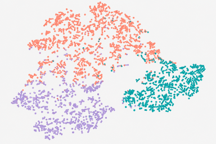
\includegraphics[width=0.45\linewidth]{figure/ACM_clusters.png}
    \caption{t-SNE visualization of learned ACM paper embeddings. Each point represents one paper, and color denotes its class.}
    \label{fig:clustering-acm}
\end{figure}

\begin{figure}[htbp]
    \centering
    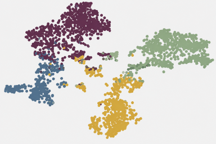
\includegraphics[width=0.45\linewidth]{figure/DBLP_clusters.png}
    \caption{t-SNE visualization of learned DBLP author embeddings. Each point represents one author, and color denotes its research area.}
    \label{fig:clustering-dblp}
\end{figure}

\begin{table}[htbp]
  \centering
  \caption{Additional clustering-quality diagnostics on DBLP and ACM,
  reported as mean $\pm$ standard deviation over five runs. Best mean
  values are bold.}
  \label{tab:clustering-diagnostic}
  \scriptsize
  \setlength{\tabcolsep}{2.5pt}
  \resizebox{\columnwidth}{!}{%
  \begin{tabular}{llcccc}
    \toprule
    & & \multicolumn{2}{c}{DBLP} & \multicolumn{2}{c}{ACM} \\
    \cmidrule(lr){3-4}
    \cmidrule(lr){5-6}
    \textbf{Group} & \textbf{Model}
    & NMI & ARI
    & NMI & ARI \\
    \midrule

    Hom./hom.
    & GAT
    & $71.50 \pm 0.36$
    & $77.26 \pm 0.48$
    & $57.22 \pm 0.19$
    & $60.47 \pm 0.31$ \\
    \midrule

    \multirow{2}{*}{Hom./het.}
    & NSD
    & $80.21 \pm 0.62$
    & $84.04 \pm 0.43$
    & $62.56 \pm 0.37$
    & $65.02 \pm 0.28$ \\

    & CSNN
    & $81.72 \pm 0.39$
    & $84.25 \pm 0.55$
    & $69.28 \pm 0.45$
    & $71.10 \pm 0.34$ \\
    \midrule

    \multirow{2}{*}{Het./hom.}
    & HAN
    & $79.12 \pm 0.47$
    & $84.76 \pm 0.58$
    & $60.63 \pm 0.22$
    & $64.28 \pm 0.41$ \\

    & PSHGCN
    & $80.38 \pm 0.52$
    & $82.65 \pm 0.36$
    & $71.89 \pm 0.49$
    & $74.31 \pm 0.57$ \\
    \midrule

    \multirow{2}{*}{Het./het.}
    & Hetero$^2$Net
    & $80.54 \pm 0.33$
    & $84.98 \pm 0.46$
    & $70.14 \pm 0.40$
    & $73.42 \pm 0.51$ \\

    & LatGRL
    & $81.36 \pm 0.56$
    & $86.07 \pm 0.38$
    & $72.52 \pm 0.61$
    & $76.75 \pm 0.44$ \\
    \midrule

    Ours
    & \textbf{\method{}}
    & $\mathbf{82.41 \pm 0.35}$
    & $\mathbf{86.52 \pm 0.42}$
    & $\mathbf{75.78 \pm 0.37}$
    & $\mathbf{78.29 \pm 0.31}$ \\
    \bottomrule
  \end{tabular}
  }
\end{table}
\section{Visualization of Node Embedding Separability During Training}
\label{sec:diffusion-process-analysis}

We further inspected the training dynamics of \method{} on the controlled four-class
\texttt{FakeHeteroDataset} from PyTorch Geometric \cite{FeyPyG2019,FeyPyG2025}. The model was trained with the default
synthetic-data settings, and the visualization includes only labeled nodes. We recorded the node
embeddings every ten epochs. As shown in Figure~\ref{fig:fakehetero-diffusion-process}, nodes from
different classes are strongly interleaved at the beginning of training. As training proceeds, the
projected embeddings of nodes in the same class form increasingly compact and separated regions. This
observation suggests that training \method{} produces more class-separable node representations on
this controlled dataset.

\begin{figure}[htbp]
   \centering
   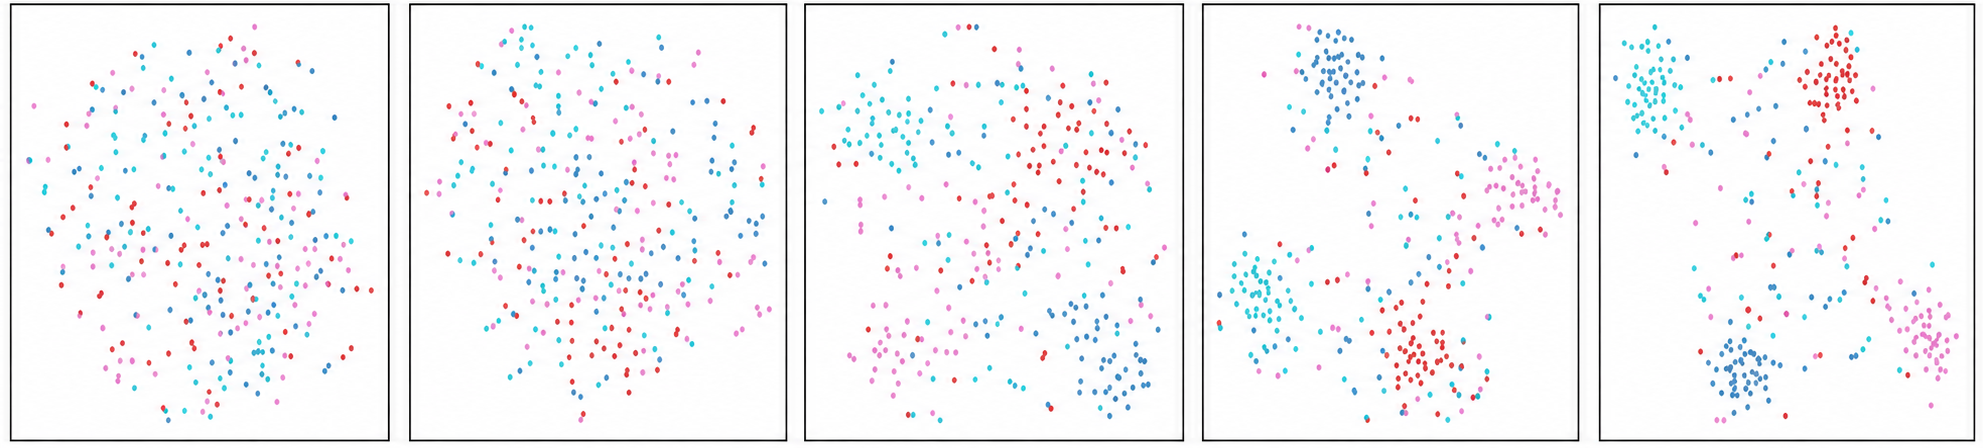
\includegraphics[width=\linewidth]{figure/model_interpret.png}
   \caption{Qualitative visualization of node embedding dynamics during training on
the four-class \texttt{FakeHeteroDataset}.}
  \label{fig:fakehetero-diffusion-process}
\end{figure}


\section{Computational Efficiency}

To characterize the computational cost, we analyze the \method{} model, the
\ampss{} component, and the \sheafcovpool{} readout.

Let \(N=|V|\) and \(M=|E|\) denote the numbers of nodes and observed directed
edges. Let \(N_{\mathrm{inst}}\) be the number of retained concrete path instances.
Define the number of boundary incidences by
\[
I_{\mathrm{bnd}}=\sum_{f\in\mathcal{I}_{\mathrm{ret}}}(\ell_f+1).
\]
Each instance contributes one closure \(1\)-cell in addition to its path edges.
Let \(\widetilde M=M+N_{\mathrm{inst}}\) denote the size of the extended edge domain.
We use \(d\) for the stalk dimension and \(K\) for the number of diffusion
steps.

\paragraph{\ampss{}.}
Stage I runs once before training. Let \(C_\Sigma\) be the number of viable
schemas, \(S_{\max}\) the selection limit, \(N_p\) the number of probe examples,
\(B\) the feature width per schema, \(C_y\) the number of classes, and \(R_{\mathrm{sel}}\)
the number of probe iterations. Greedy selection evaluates
\(O(C_\Sigma S_{\max})\) subsets whose feature width grows to \(S_{\max}B\), giving
\[
O(R_{\mathrm{sel}}N_pBC_yC_\Sigma S_{\max}^2)
\]
probe time. Label propagation and schema/path enumeration additionally cost
\(O(K_{\mathrm{LP}}(M+N)C_y+Q_{\mathrm{type}}+Q_{\mathrm{samp}})\), where
\(K_{\mathrm{LP}}\) is the number of label-propagation iterations and the \(Q\) terms
count the visited typed and concrete path prefixes. Sparse coverage and
schema features require
\[
O(C_\Sigma L_{\max}+N_pS_{\max}B+N_{\mathrm{cov}}+I_{\mathrm{bnd}})
\]
storage, where \(L_{\max}\) is the maximum schema length and \(N_{\mathrm{cov}}\) is the
number of stored coverage entries. Stage II adds
\(O(N_{\mathrm{inst}}(h_f+d_r)h_\beta)\) instance-weighting time, where \(h_f\) is the
ordered-path latent width and \(h_\beta\) is the weighting-network width. The positive weights
do not prune operator tensors.

\paragraph{\method{}.}
To construct the scaled-orthogonal restriction maps, we use the Fast
Householder Product parameterization~\cite{mathiasen2020fasth}. Node-to-edge
maps are learned only for the \(M\) observed edges, whereas closure and
edge-to-face maps are obtained by path transport. Their dense
\(d\times d\) matrix operations require \(O((M+I_{\mathrm{bnd}})d^3)\) construction time.
The resulting maps are cached across diffusion steps, requiring
\(O((\widetilde M+I_{\mathrm{bnd}})d^2)\) space. Thus, map construction is cubic in the
stalk dimension, while memory grows quadratically.
Each matrix-free diffusion step applies the node-mediated and face-induced
components of the edge operator in
\[
O\!\left((\widetilde M+I_{\mathrm{bnd}})d^2+(N+\widetilde M)d\right)
\]
time. Hence, when the MLP widths and \(d_r\) scale with \(d\), the backbone
costs
\[
O\!\left(
Nd_{\mathrm{in}}d+(M+I_{\mathrm{bnd}})d^3
+K\bigl[(\widetilde M+I_{\mathrm{bnd}})d^2+(N+\widetilde M)d\bigr]
\right)
\]
time and
\[
O\!\left((\widetilde M+I_{\mathrm{bnd}})d^2+(N+\widetilde M+I_{\mathrm{bnd}})d\right)
\]
inference space. For fixed \(d\) and \(K\), both costs are linear in the
graph size and retained boundary incidences; no dense Laplacian is formed.

\paragraph{\sheafcovpool{}.}
With three node/edge views, projected dimension \(d_p\), pooling width \(h_p\),
\(N_{\mathrm{graph}}\) graphs, and \(C_{\mathrm{cls}}\) classes, the readout costs
\[
O\!\left(
\widetilde M d^2
+(N+\widetilde M)(d+h_pd_p+d_p^2)
+N_{\mathrm{graph}}(h_pd_p^2+h_pC_{\mathrm{cls}})
\right)
\]
time and
\[
O\!\left((N+\widetilde M)(d+d_p^2)+N_{\mathrm{graph}}d_p^2\right)
\]
space. The \(\widetilde M d^2\) term transports extended-edge states into
their endpoint stalks. With fixed dimensions, \sheafcovpool{} is linear in
the extended graph size and constructs neither a dense node-to-node
covariance matrix nor a coarsened graph.

Table~\ref{tab:efficiency} reports the measured runtime, parameter count, and memory usage on the
ACM node-classification task.

\begin{table}[htbp]
  \centering
  \caption{Efficiency comparison on ACM. Best values are bold. HetSheaf's code is unavailable, so we use the results reported for the HetSheaf ensemble model in the original paper.}
  \label{tab:efficiency}
  \scriptsize
  \begin{tabular}{lccc}
    \toprule
    \textbf{Model} & Runtime (s) & Parameters & Memory (MB) \\
    \midrule
    HAN & 28.9 & 2.2M & 1{,}780 \\
    HGT & 1{,}025.8 & 7.2M & 6{,}120 \\
    NSD & 47.6 & \textbf{155K} & \textbf{980} \\
    HetSheaf & 55.7 & 174K & - \\
    \midrule
    \textbf{\method{}} & 72.1 & 517K & 1120 \\
    \bottomrule
  \end{tabular}
\end{table}

Table~\ref{tab:efficiency} shows that \method{} requires more parameters, more memory, and has a higher runtime than other models including HetSheaf, the closest heterogeneous sheaf baseline. This is because \method{} retains path-supported \(2D\)-cells and performs sheaf-Hodge diffusion on both node and edge cochains, which increases the computational cost. However, \method{} achieves better performance than all baselines, as shown in Table~\ref{tab:node-cls}, Table~\ref{tab:link-pred}, and Table~\ref{tab:graph-cls}. This suggests that the additional computational cost of \method{} is justified by its superior performance.

\end{document}
